

\setcounter{chapter}{10-1} %Makes the prereq chapter chapter 0

\chapter{Recurrent Neural Networks}

    This chapter was originally placed immediately after the Convolutional Neural Networks Chapter.

    \begin{itemize}
        \item Additionally, this chapter relies on having read the State Machines section of the Markov Decision Process (MDP 0).
    \end{itemize}

    \subsection{Review: Neural Networks So Far}

        In this class, we design \textbf{models} we can \textbf{train} to handle different tasks.
        
        All of this has culminated in the \vocab{neural network}: a model class that can handle a huge number of interesting problems.
        
            \begin{itemize}
                \item To create a neural network, we combine many smaller, simpler models together in a systematic, \gren{non-linear} way.
                    \note{Remember that by "systematic", we mostly just mean "organized":
                    
                    \phantom{}
                    
                    The parts of our model are cleanly organized, to make our math easier.}

                \item This creates the "\vocab{fully connected}" (FC) neural network.
            \end{itemize}
        
        We then discovered a \textit{weakness} of FC neural networks: they don't understand \orgg{space} very well! 
            \begin{itemize}
                \item \miniex FC networks don't encode information about which pixels are \textbf{close} or \textbf{far} from each other.
            \end{itemize}
            
        Our solution was the \vocab{convolutional neural network} (CNN): 
        \begin{itemize}
            \item We used \gren{convolution} as a way to represent which elements were "near" each other in space.
        \end{itemize}




    \phantom{}
        
    \subsection{Time in a Neural Network}
    
        We've created models that can model \textit{space}. We might also wonder: can we make it so they understand \orgg{time}, as well?

        Right now, our neural networks have no built-in way to \textit{represent} time: each data point stands by itself.
            \note{Note that we're focused on the \textbf{finished} model:
            
            \phantom{}
            
            The model changes while training, but the fully-trained model \textbf{doesn't} keep track of the past.}

        \begin{itemize}
            \item As we discussed in the CNN chapter, the \purp{order} of our input variables is mostly \textbf{ignored} by the model.\\
        \end{itemize}

        \begin{concept}
            A traditional, fully connected \gren{neural network} cannot easily use information about \vocab{time}, or the \purp{past}.
        \end{concept}

        Previously, we added structure to NNs using \textbf{convolution}. But this \textit{doesn't} work as well in time as it does in space:\\

        \begin{concept}
            \vocab{Time} and \purp{space} behave differently:
            
            \begin{itemize}
                \item Information can be spread out over \orgg{any direction} in space.
                \item However, information only travels \gren{forward}, not backward, in time.
            \end{itemize}

            So, we need to model them differently.
        \end{concept}
        
        Realistically, we want model that can keep track of time, and order of past events, for plenty of purposes:

        \begin{itemize}
            \item \miniex Stocks, weather, choosing the best plan of action, etc.
                \begin{itemize}
                    \item "It rained yesterday" and "it rained last week" have very different effects on today's weather.
                \end{itemize}
        \end{itemize}
        


    \phantom{}
        


\pagebreak

\section{State Machines}

    \textit{This section is identical to the notes from MDP 0. If you have already read that section, skip to C.2.}

    \iffalse


    \subsection{How to Model Time}

        How do we want to model time?

        The simplest way is one we've used before: keeping track of the current \gren{timestep} $t$.

        \begin{itemize}
            \item But this is too little information to be useful: it doesn't tell us much.
            \item \miniex If I told you "the current time is $t=1563$", that doesn't help you much with decision-making.
        \end{itemize}

        So, what would be a \textbf{useful} representation of time? We've already shown that we don't really care much about the exact \textbf{index} of time $t$.

        Instead, we care about \gren{what happened} in the past.\\

        \begin{concept}
            One simple way to record the past is to ask about \gren{events}, and \purp{when} they happened.
        \end{concept}

        \miniex You might keep track of a medical history, or the purchases made by a company over the last year.


    \phantom{}

    \subsection{States}

        Keeping a "history" of events is an \textbf{improvement}. In some contexts, though, it can become \textbf{expensive}: the \textbf{longer} our time frame, the more events will pile up.

        We could ignore very \gren{old} events, but whether an old event matters depends on the context.

        \begin{itemize}
            \item \miniex If we omit all company profits/expenses from more than 3 years ago, we don't know our balance. What if we forgot a debt?
        \end{itemize}

        This particular example has a pretty simple solution: just keep track of the \gren{total} amount of money you have.

        And herein lies our \textit{general} solution: rather than keeping track of every single event, we can keep track of the \redd{state} that result from those past events.\\

        \begin{definition}
            A \vocab{state} represents information we use to keep track of the \purp{current situation} you're in.
            
            It allows us to store "\gren{memory}" about the past:

            \begin{itemize}
                \item If an event changes our current situation, we'll \orgg{update} the state.
                \item Then, in future timesteps, we'll use that updated state.
            \end{itemize}

            \subsecdiv
            
            A state can be almost \purp{any information} that we want to keep.

            \begin{itemize}
                \item In practice, we want to exclude unhelpful, irrelevant, or outdated data.
            \end{itemize}
        \end{definition}

        \miniex Suppose that you're an investor. Your state could include: 1. how much money you have, 2. the stocks you current own, and 3. whether the market seems to be going up or down.

        \begin{itemize}
            \item Notice that, while these variables don't give you exact time, they do \textbf{remember} past events: if you have $\$30$, you at some point must have gotten those $\$30$.
        \end{itemize}
        
        There are many other kinds of states: position and velocity of an object, or the progress on a project, etc.




    \phantom{}

    \subsection{How states are stored}

        Now that we've introduced the idea, we'll start formally notating it.\\

        \begin{notation}
            Typically, a \vocab{state} \red{$s$} stores our information as a \purp{vector}.
            
            We represent the \textbf{set} of all possible \redd{states} as \red{$\mathcal{S}$}. 
            
            \begin{itemize}
                \item We can have a \textbf{finite} or \textbf{infinite} set of states, depending on the situation.
                \item If $s$ is one of our states, we can express that as \red{$s \in S$}.
            \end{itemize}

            \subsecdiv
            
            Our state at time $t$ is \red{$s_t$}.
            
            Our \vocab{initial state} ($t=0$) is represented as \red{$s_0$}.         
            \begin{itemize}
                \item Since it's a state, $s_0 \in \mathcal{S}$.
            \end{itemize}
        \end{notation}

        We now have two of the pieces of our state machine:
            
        \begin{itemize}
            \item $\red{\mathcal{S}}$ is a finite or infinite \textbf{set} of possible \textbf{states} \red{$s$}.
            \item $\red{s_0 \in \mathcal{S}}$ is the \textbf{initial state} of the machine. 
        \end{itemize}




    \phantom{}

    \subsection{State examples}
        Let's show a couple examples of what states different systems might have.
            \note{There are multiple different ways to represent the same set of states with a vector, so we won't specify the representation.}
        
        \begin{itemize}
            \item The game of chess.
                \begin{itemize}
                    \item The \textbf{finite} set \red{$S$} is the set containing \redd{every chess board}.
                    \item The initial state \blu{$s_0$} is the \vocab{board} when you first \vocab{start playing}.
                \end{itemize}
                
            \item A ball moving in space, with coordinates.
                \begin{itemize}
                    \item The \textbf{infinite} set \red{$S$} contains \redd{every pair 
                    $ \Big[\text{position},\text{velocity} \Big]$}
                    for the ball.
                        \begin{itemize}
                            \item For example, the ball might be in state $\Big[ (1,2), (5,0)\Big]$:
                            \item at position $(1,2)$, 
                            \item with velocity $(5,0)$.
                            
                        \end{itemize}
                    \item The initial state \blu{$s_0$} is the \vocab{position and velocity} when you first \vocab{release} the ball.
                \end{itemize}
                
            \item A combination lock with 3 digits.
                \begin{itemize}
                    \item The \textbf{finite} set \red{$S$} contains every \redd{sequence of 3 digits}, where only one sequence unlocks the lock.
                        \begin{itemize}
                            \item For example: $[0,0,0]$, \; $[4,6,9]$, \; $[9, 0, 2]$, \; etc.
                        \end{itemize}
                    \item The initial state \vocab{$s_0$} is the \blu{sequence} when you \vocab{leave} your lock; maybe $[1,2,3]$.
                \end{itemize}
        \end{itemize}




    \pagebreak

    \subsection{Input}

        We now have a way to \textbf{store} our information in time. However, we need to know how to \textbf{update} our state: what happens if we learn new information? 

        We'll include some new variables to address this.

        \subsecdiv

        At each timestep, we get some kind of \textbf{input} $x$, which is our update: this is the newest information about our system. We'll \textit{also} store this in a vector.\\
        
        \begin{definition}
            The \vocab{input} \bru{$x$} represents \purp{new information} we get from our system.
            
            We represent the \textbf{set} of all possible \brun{inputs} as \bru{$\mathcal{X}$}.
                \begin{itemize}
                    \item This set can be \textbf{finite} or \textbf{infinite}.
                    \item We can say \bru{$x \in \mathcal{X}$}.
                \end{itemize}
                
            Our input at time $t$ is \bru{$x_t$}.
        \end{definition}




    \phantom{}

    \subsection{Transition}

        Based on this new information, we need update the current \gren{state} of the world.

        \begin{itemize}
            \item But often, this update depends both the new information, \textbf{and} the \gren{old state}.
        \end{itemize}

        \miniex If your timestep update tells you "got 50 dollars", you need to know how much money you had before, to get your new total.

        \begin{equation}
            \overbrace{\red{s_{t+1}}}^{\text{New balance}} = 
            \overbrace{\red{s_t}}^{\text{Old balance}} + 
            \overbrace{\bru{x_t}}^{\text{Money added}}
        \end{equation}

        \subsecdiv

        Here's a second example.

        \miniex Suppose you're taking care of a plant.

        \begin{itemize}
            \item If a plant is dry ($s_t=$ Dry), then watering it will make it healthier ($s_{t+1}=$ Healthy).
            \item If the plant is watered ($s_t=$ Healthy), then watering it more might make it sick ($s_{t+1}=$ Sick).
        \end{itemize}
            
        We're \textbf{transitioning} between states, so we use a \textbf{transition function}.\\
        
        \begin{definition}
            The \vocab{transition function} \gren{$f_s$} tells us how to update our \redd{state}, based on our new \brun{input} information.

            \begin{itemize}
                \item Thus, our transition takes in two pieces of information: \red{$s$} and \bru{$x$}.
            \end{itemize}
            
            
            
            \begin{equation*}
                \grn{f_s}(\red{s},\bru{x})
            \end{equation*}

            \begin{itemize}
                \item We use this function at \purp{every timestep} $t$ to get our next state, at time $t+1$.
            \end{itemize}
            
            
            \begin{equation*}
                \grn{f_s}(\red{s_t},\bru{x_t}) = \red{s_{t+1}}
            \end{equation*}

            \subsecdiv
            
            We can treat each state-input \purp{pair} as an object, $(s,x)$. Thus, the set of all of these pairs is $\mathcal{S} \cross \mathcal{X}$.
            
            \begin{equation*}
                \grn{f_s}: \red{\mathcal{S}} \cross \bru{\mathcal{X}} 
                \rightarrow \red{\mathcal{S}}
            \end{equation*}
        \end{definition}

        We can visualize this as:
    
        \begin{figure}[H]
            \centering
            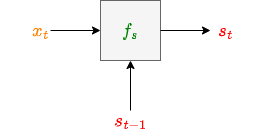
\includegraphics[width=60mm,scale=0.4]{images/rnn_images/transition_diagram.png}
        \end{figure}

        Now, we have two more pieces of our state machine:
        
        \begin{itemize}
            \item \bru{$\mathcal{X}$} is a finite or infinite set of possible \textbf{inputs} \bru{$x$}.
            \item \grn{$f_s$} is the \textbf{transition function}, which moves us from one state to the next, based on the input.
                \begin{equation}
                    \grn{f_s}: \red{\mathcal{S}} \cross \bru{\mathcal{X}} 
                    \rightarrow \red{\mathcal{S}}
                \end{equation}
        \end{itemize}



    \phantom{}

    \subsection{Transition Examples}
        
        Now, we revisit our examples, and consider how they "transition":
        
        \begin{itemize}
            \item The game of chess.
                \begin{itemize}
                    \item The input \bru{$x$} is the \brun{choice} our player makes, \brun{moving one piece} on the chess board according to the \textbf{rules}.
                    
                    \item The transition function \grn{$f_s$} applies this move to our current chess board, and produces a \gren{new chess board}.
                        \begin{itemize}
                            \item If we moved our pawn, the transition function outputs the board \gren{after} that pawn is \gren{moved}.
                        \end{itemize}
                \end{itemize}
                
            \item A ball moving in space, with coordinates.
                \begin{itemize}
                    \item The input \bru{$x$} might represent a \brun{push} changing the ball's velocity.
                    
                    \item The transition function \grn{$f_s$} uses the push to change our \brun{velocity}, and the velocity to change the ball's \brun{position}.
                        \begin{itemize}
                            \item If our ball wasn't moving before, and we \gren{push} it, the new state is \gren{moving} in that direction.
                        \end{itemize}
                \end{itemize}
                
            \item A combination lock with 3 digits.
                \begin{itemize}
                    \item The input \bru{$x$} is you \brun{changing} one of the three digits on the lock: for example, \brun{increasing} the first digit by 3.
                    
                    \item The transition function \grn{$f_s$} applies the \gren{change} you make to the lock.
                        \begin{itemize}
                            \item If the first digit was 2, and you \gren{increase} it by 3, the new first digit is 5.
                        \end{itemize}
                \end{itemize}
        \end{itemize}




    \pagebreak
        
    \subsection{Output}
        
        We now have a system for keeping \textbf{track} of our state, and \textbf{updating} that state: this is a really powerful tool for managing time!
        
        We're still missing something, though: why do we \textbf{care} about our state? Typically, there's some \textbf{result} we actually want from storing our state.
            \note{Just like how in CNNs, convolution wasn't the end goal: it was a transformation to help improve regression/classification.}

        \subsecdiv
        
        Usually, the desired output is more simple than keeping track of everything we want to \textbf{remember}.
            
        \miniex If we're storing a bunch of information about the stock market, and our own money, we might simply return "invest in $X$" or "do not invest in $X$".
        
        The is what we call our \textbf{output}.\\
        
        \begin{definition}
            The \vocab{output} \purp{$y$} represents the \purp{result of our current state}. 
            
            What we use as "output" depends on what we are \gren{trying to predict/compute}.
            
                \begin{itemize}
                    \item Sometimes, the output is the \textbf{only} thing (aside from input) we can \textbf{see}. This happens when the state is \vocab{hidden}!
                \end{itemize}

            \subsecdiv
            
            In other words, while the state \gren{stores} relevant information to keep track of the situation, the \purp{output} is the decision based on this information.
            
            We represent the \textbf{set} of all possible \purp{outputs} as \purp{$\mathcal{Y}$}.
            
            \begin{itemize}
                \item This set can be \textbf{finite} or \textbf{infinite}.
                \item If $y$ is a possible output, we say \purp{$y \in \mathcal{Y}$}.
            \end{itemize}
                
            Our output at time $t$ is \purp{$y_t$}.
        \end{definition}

        Note that we use $y_t$: we don't necessary create a single output at the end of our runtime.
        
        \begin{itemize}
            \item Instead, we continuously create outputs at each timestep.
        \end{itemize}



    \phantom{}

    \subsection{Output Function}
        
        So now, we need to actually \textbf{compute} our output. This will be based on all the data we have \gren{stored} at the time we're asked for an output.

        \begin{itemize}
            \item We don't need to use the input, because the input data is already included in the state.
        \end{itemize}

        We can create an output for each timestep using the \purp{output function}.\\

        \begin{definition}
            The \vocab{output function} \grn{$f_o$} tells us what \purp{output} we get based on our current \redd{state}.
            
            Thus, our \gren{output function} only takes in the \redd{state}. 
            
            \begin{equation*}
                \grn{f_o}(\red{s_t}) = \pur{y_t}
            \end{equation*}
            
            It uses our current information (\redd{state}) to produce a the result we're interested in (\purp{output}).
            
            Using sets, we can write this as:
            
            \begin{equation*}
                \grn{f_o}: \red{\mathcal{S}} \rightarrow \pur{\mathcal{Y}}
            \end{equation*}
        \end{definition}
        
        We visualize this unit as:
        
        \begin{figure}[H]
            \centering
            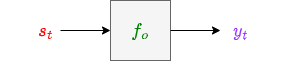
\includegraphics[width=60mm,scale=0.4]{images/rnn_images/output_diagram.png}
        \end{figure}

        This gives us the last two parts of our state machine:
            
        \begin{itemize}
            \item \purp{$\mathcal{Y}$} is a finite or infinite set of possible \textbf{outputs} \purp{$y$}.
            
            \item \grn{$f_o$} is an \textbf{output function}, which gives us our output based on our state.
                \begin{equation}
                    \grn{f_o}: \red{\mathcal{S}} \rightarrow \pur{\mathcal{Y}}
                \end{equation}
        \end{itemize}



    \phantom{}
    
    \subsection{Output Examples}
        
        Again, we go to our examples, and give them outputs, completing our state machines:
        
        \begin{itemize}
            \item The game of chess.
                \begin{itemize}
                    \item The output \purp{$y$} could be many things. But, what do we care about most: \purp{winning}! 
                        \begin{itemize}
                            \item So, \purp{$\mathcal{Y}$} will have four options: "ongoing", "draw", "player 1 win", "player 2 win".
                        \end{itemize}
                        
                    \item The output function \grn{$f_o$} will give us our output. Thus, it represents the \gren{chess rules} for whether there is a winner or a draw.  
                        \begin{itemize}
                            \item So, \grn{$f_o$} looks at a board, and tells us whether someone has won, or there's a draw.
                        \end{itemize}
                \end{itemize}
                
            \item A ball moving in space, with coordinates.
                \begin{itemize}
                    \item We want output \pur{$y$}.
                        \begin{itemize}
                            \item Sometimes, the \purp{output} is the same as the \redd{state}: all we want to know is what's \textbf{happening}!
                            
                            \item In this case, we'll say our \textbf{output is the state}: we return the \purp{position} and \purp{velocity} of the ball.
                                \note{We could have chosen a different output if we had a specific goal in mind!}
                        \end{itemize}
                        
                    \item If our state and output are the same, then the output function \grn{$f_o$} should just \gren{copy} the state it receives!
                        \begin{itemize}
                            \item Our function is the \vocab{identity function}: $\grn{f_o}(\red{s}) = \red{s}$.
                        \end{itemize}
                \end{itemize}
                
            \item A combination lock with 3 digits.
                \begin{itemize}
                    \item We want our output \purp{$y$}. 
                        \begin{itemize}
                            \item Our goal is more clear: we want the combination lock to be \purp{open} or \purp{closed}. So, those are our outputs \purp{$\mathcal{Y}$}.
                        \end{itemize}
                        
                    \item Our function \grn{$f_o$} will tell us the lock is open if the current digits exactly \gren{match the correct sequence}.
                \end{itemize}
        \end{itemize}


    \pagebreak

    \subsection{A Completed State Machine}

        Finally, we can assemble our completed state machine.\\
        
        \begin{definition}
            A \vocab{State Machine} can be formally defined as a collection of several objects 
            
            \begin{equation*}
                (\red{\mathcal{S}}, \bru{\mathcal{X}}, \pur{\mathcal{Y}}, 
                \red{s_0}, \grn{f_s}, \grn{f_o})
            \end{equation*}
            
            We have three sets:
            
            \begin{itemize}
                \item $\red{\mathcal{S}}$ is a finite or infinite \textbf{set} of possible \textbf{states} \red{$s$}.
                
                \item $\bru{\mathcal{X}}$ is a finite or infinite \textbf{set} of possible \textbf{inputs} \bru{$x$}.
                
                \item $\pur{\mathcal{Y}}$ is a finite or infinite \textbf{set} of possible \textbf{outputs} \purp{$y$}.
            \end{itemize}
            
            And components to allow us to transition through time:
            
            \begin{itemize}
                \item $\red{s_0 \in \mathcal{S}}$ is the \textbf{initial state} of the machine. 
                
                \item \grn{$f_s$} is the \textbf{transition function}, which moves us from one state to the next, based on the input.
                    \begin{equation*}
                        \grn{f_s}: \red{\mathcal{S}} \times \bru{\mathcal{X}}
                        \rightarrow \red{\mathcal{S}}
                    \end{equation*}

                \item \grn{$f_o$} is an \textbf{output function}, which gives us our output based on our state.
                    \begin{equation*}
                        \grn{f_o}: \red{\mathcal{S}} \rightarrow \pur{\mathcal{Y}}
                    \end{equation*}
            \end{itemize}
        \end{definition}
        
        We have:
        
        \begin{itemize}
            \item Our \redd{state} to store information,
            \item Our \brun{input} to update information,
            \item Our \purp{output} gives us the result of our information.
        \end{itemize}
        
        And to combine these, we need:
        
        \begin{itemize}
            \item Our \vocab{initial} state,
            \item How to \gren{change} states,
            \item How to \gren{get} an \gren{output}.
        \end{itemize}



    \phantom{}

    \subsection{Using a State Machine}

        How do we work with a state machine? Well, we have all of the tools we need.
        
        We start with out initial state, $\red{s_0}$. For our \textbf{first} timestep, we get a new input: new \textbf{information}. We use this to get a new state.
        
        \begin{equation}
            \red{s_1} = 
            \grn{f_s}(\red{s_0}, \bru{x_1})
        \end{equation}
        
        With this state, we can now get our \textbf{output}.
        
        \begin{equation}
            \pur{y_1} = 
            \grn{f_0}(\red{s_1})
        \end{equation}
        
        We've calculated everything in our \textbf{first} timestep! Now, we can move on to our \textbf{second} timestep, and do the same thing.
        
        In general, we'll repeatedly follow the process:
        
        \begin{equation}
            \red{s_t} = 
            \grn{f_s}(\red{s_{t-1}}, \bru{x_t})
        \end{equation}
        
        \begin{equation}
            \pur{y_t} = 
            \grn{f_o}(\red{s_t})
        \end{equation}
        
        
        \begin{concept}
            To move through time in a state machine, we follow these steps from $t=1$:
            
            \begin{itemize}
                \item Use the \bru{input} and \red{state} to get our \red{new state}.
                    \begin{equation*}
                        \red{s_t} = 
                        \grn{f_s}(\red{s_{t-1}}, \bru{x_t})
                    \end{equation*}
                    
                \item Use the \red{new state} to get our \pur{output}.
                    \begin{equation*}
                        \pur{y_t} = 
                        \grn{f_o}(\red{s_t})
                    \end{equation*}
                    
                \item Increment the time from $t$ to $t+1$.
                
                    \begin{equation*}
                        t_{new} = t_{old} + 1
                    \end{equation*}
                
                \item Repeat.
            \end{itemize}
        \end{concept}



    \phantom{}

    \subsection{Example Run-Through of a State Machine}

        To make this more concrete, we'll build our own simple state machine and run a couple iteration steps.
                
        Suppose you're saving up money to buy something. At each timestep, you gain or lose some money. 
        
        You want to know when you have enough money to buy it. 
            \note{This example is simple enough that you might feel like a state machine is unnecessary. However, this is just for demonstration!}
            
        What are each of the parts of our state machine?
        
        \begin{itemize}
            \item The state $\red{s}$: how much money do we have right now?
            
            \item The input $\bru{x}$: the money we add to our savings.
            
            \item The output $\pur{y}$: we want to know when we have enough money. Maybe our goal is 10 dollars.
            
            \item Initial $\red{s_0}$: we start with 0 dollars.
            
            \item Transition $\grn{f_s}$: we just add the new money to how much we have saved up.
            
                \begin{equation}
                    f_s(\red{s},\bru{x}) = \red{s}+\bru{x}
                \end{equation}
                
            \item Output $\grn{f_o}$: do we have enough money?
            
                \begin{equation}
                    \grn{f_o}(\red{s}) = (\red{s} \geq 10)
                    =
                    \begin{cases}
                        \text{True} & \text{If } s \geq 10 \\
                        \text{False} & \text{Otherwise}
                    \end{cases}
                \end{equation}
        \end{itemize}
        
        We'll run through our state machine for the following input:
        
        \begin{equation}
            \red{X} = [x_1, \; x_2, \; x_3, \; x_4] = [ 4, \; 5, \; 6, \; -7]
        \end{equation}
        
        Let's apply the steps above:
        
        \begin{itemize}
            \item Get new state from (old state, input).
            \item Get output from new state.
            \item Increment time counter.
        \end{itemize}
        
        For our first step, we get:
        
        \begin{equation}
            \begin{matrix}
                \red{s_1} = 4+0 = \red{4} \\
                \\
                \pur{y_1} = ( 4 \geq 10 ) = \text{\pur{False}}
            \end{matrix}
        \end{equation}
        
        For the others, we get:
        
        \begin{equation}
            \begin{matrix}
                \red{s_2} = 9 \\ \pur{y_2} = \text{False}
            \end{matrix}
            \;\; \longrightarrow \;\; 
            \begin{matrix}
                \red{s_3} = 15 \\ \pur{y_3} = \text{True}
            \end{matrix}
            \;\; \longrightarrow \;\; 
            \begin{matrix}
                \red{s_4} = 8 \\ \pur{y_4} = \text{False}
            \end{matrix}
        \end{equation}
        
        Though our transition and output functions might become more complicated, this is the basic idea behind all state machines.




    \phantom{}

    \subsection{State Machine Diagram}
    
        Finally, we'll create a visualization that represents our state diagram.
        
        \subsubsection{Transition Function}
        
            Our \grn{transition function} follows this format:
            
            \begin{equation}
                \red{s_t} = 
                \grn{f_s}(\red{s_{t-1}}, \bru{x_t})
            \end{equation}
            
            We can diagram this component as:
            
            \begin{figure}[H]
                \centering
                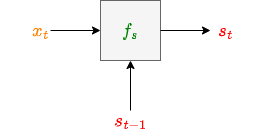
\includegraphics[width=60mm,scale=0.4]{images/rnn_images/transition_diagram.png}
            \end{figure}
            
            Note that the state appears \purp{twice}: once as an input, once as an output.
            
            In the \textit{next} timestep, $s_t$ will be the \textbf{input} to $f_s$, even though it's currently the \textbf{output}.
                \note{If $t=10$, then $s_{10}$ is the output. If $t=11$, then $s_{10}$ is the input!}

            \begin{itemize}
                \item We'll create a way to represent this later.
            \end{itemize}
            
        
        \subsecdiv
        
        \subsubsection{Output Function}
        
            Our \gren{output function} takes in the state we just got from the transition function:
            
            \begin{equation}
                \pur{y_t} = 
                \grn{f_o}(\red{s_t})
            \end{equation}
            
            So, we diagram it accordingly:
            
            \begin{figure}[H]
                \centering
                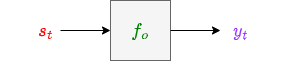
\includegraphics[width=60mm,scale=0.4]{images/rnn_images/output_diagram.png}
            \end{figure}
            
            As we mentioned, the \textbf{output} function takes in the state as its input. 
            
            \begin{itemize}
                \item That means that the \redd{output} of $f_s$, is the \redd{input} of $f_o$.
            \end{itemize}
            
            \begin{figure}[H]
                \centering
                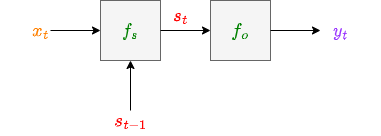
\includegraphics[width=80mm,scale=0.4]{images/rnn_images/state_machine_protodiagram.png}
            \end{figure}
            
        \subsecdiv
        
        \subsubsection{Time Delay}
        
            Only one thing is missing: we know that our current state $\red{s_t}$ needs to be reused \textbf{later}: we'll need it to compute our \textit{new} state $\red{s_{t+1}}$.
            
            We don't want it to \textit{immediately} send the state information back to $f_s$: we only use the function once per timestep. So, we'll \textit{delay} by waiting one time step.
            
            We'll use a little clock symbol to represent this fact.
            
            \begin{figure}[H]
                \centering
                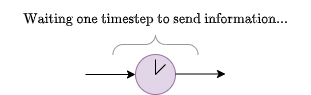
\includegraphics[width=80mm,scale=0.4]{images/rnn_images/clock.png}
            \end{figure}
            
            \begin{notation}
                We can depict a \vocab{state machine} using the following diagram:
                
                \begin{figure}[H]
                    \centering
                    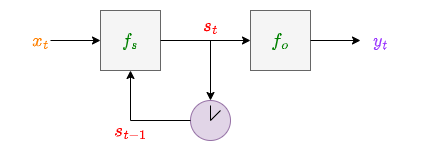
\includegraphics[width=90mm,scale=0.4]{images/rnn_images/state_machine_diagram.png}
                \end{figure}
                
                At every timestep, we use $\bru{x_t}$ and $\red{s_{t-1}}$ to calculate our new state, and our new output.
                
                The circular "clock" element represents our \purp{delay}: $\red{s_t}$ becomes the input to $f_s$ on the \purp{next} timestep.
            \end{notation}




    \pagebreak

    \subsection{Finite State Machines}

        To get used to state machines, we'll start with a simpler, special case, the \textbf{finite state machine}.\\
            
        \begin{definition}
            A \vocab{finite state machine} is a state machine where
            
            \begin{itemize}
                \item The set of states $\red{\mathcal{S}}$
                \item The set of inputs $\bru{\mathcal{X}}$
                \item The set of outputs $\pur{\mathcal{Y}}$
            \end{itemize}
            
            Are all \vocab{finite}. Meaning, the total space of our state machine is \purp{limited}.
            
            Each aspect of our state machine can be put into a finite list of elements: this often makes it easier to \textit{fully} describe our state machine.
        \end{definition}
        
        This seemingly limited tool is more powerful than it seems: \textbf{all computers} can be described as finite state machines!
            \note{Even when a computer seems to be describing "infinite" collections of things, it only has a finite amount of space to represent them.}




    \phantom{}

    \subsection{State Transition Diagrams}

        One nice thing about the simplicity of a finite state machine is that we can represent it \textbf{visually}.
            
        Let's build one up: we'll pick a simple, though not entirely realistic example.
        
        \miniex We have a blanket. It can be in three states: either \blu{wet}, \grn{dry}, or \red{burning}. We can represent each state as a "node".
        
        \begin{figure}[H]
            \centering
            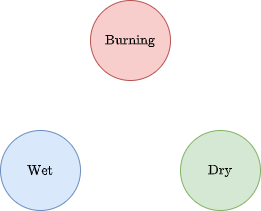
\includegraphics[width=60mm,scale=0.4]{images/rnn_images/std_states.png}
        \end{figure}
        
        \begin{concept}
            In a \vocab{state transition diagram}, states are represented as \purp{nodes}, or points on the graph.
        \end{concept}
        
        We have our states down. The other important thing is our \textbf{transitions}. How do we go between states?
        
        Well, one input could be \textbf{water}: it would stop the blanket from burning. In any case, the blanket will be wet.
        
        \begin{figure}[H]
            \centering
            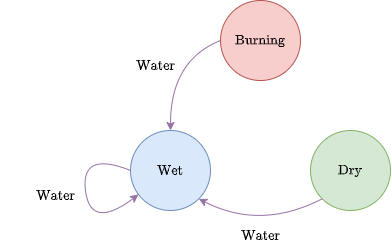
\includegraphics[width=80mm,scale=0.4]{images/rnn_images/std_water.png}
        \end{figure}
        
        Now, we can see: each arrow represents a \textbf{transition} between two states. Each \textbf{input} gets its own transition.\\
        
        \begin{concept}
            In a \vocab{state transition diagram}, transitions are represented as \purp{arrows} between states.
            
            We usually label these with whichever \brun{input} will cause that transition.
        \end{concept}
        
        Also notice that a state can transition to itself: a wet blanket \textbf{stays wet} when you add water.
        
        What if we add \textbf{fire}? That would make a dry blanket \textbf{burn}. But, we could also use it to \textbf{dry off} the wet blanket!
        
        \begin{figure}[H]
            \centering
            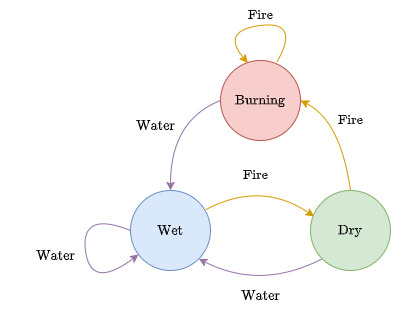
\includegraphics[width=80mm,scale=0.4]{images/rnn_images/std_fire_and_water.png}
        \end{figure}
        
        And now, we have a simple \textbf{state transition diagram}!
            \note{Note that our diagram doesn't show the output. In this case, that's not a problem: the output is the state.}
        
        Each transition, as usual, is based on two things: the \textbf{current} state (where the arrow starts) and the \textbf{input}(which arrow you follow).\\
        
        \begin{definition}
            A \vocab{state transition diagram} is a \purp{graph} of 
            
            \begin{itemize}
                \item Nodes (\red{points}) representing \red{states}
                \item Directed edges (\grn{arrows}) representing \grn{transitions}
            \end{itemize}
            
            Where each input-state pair has one arrow associated with it.
            
            These arrows show one \grn{transition}, with the properties:
            
            \begin{itemize}
                \item The start and end \red{states} represented by the start and the end of the arrow
                \item The \bru{input} that causes this transition is labelled.
            \end{itemize}
            
            This diagram does not have to show the input.
        \end{definition}
        
            \note{If you're not familiar with "nodes" or "edges", don't worry about it! For our purposes, "point" and "arrow" are good enough.}




    \phantom{}

    \subsection{Simplified state transition diagrams: One-input graphs}
        
        One more consideration: the graph above is helpful, but it's a bit \textbf{complicated}. 
        
        In fact, if we added more \textbf{states}, or more \textbf{inputs}, it could get too complicated to read!
        
        Our solution: if a system is too complicated, we create a separate state-transition diagram for \textbf{each input}.
        
        \begin{figure}[H]
            \centering
            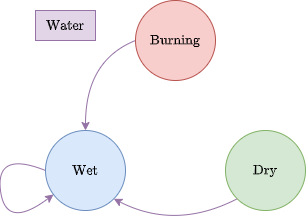
\includegraphics[width=60mm,scale=0.4]{images/rnn_images/std_water_no_label.png}
            \qquad
            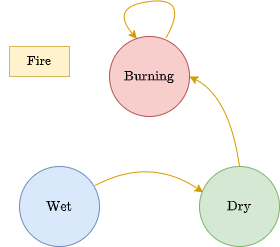
\includegraphics[width=55mm,scale=0.4]{images/rnn_images/std_fire.png}
            
            \caption*{The left diagram only uses \textbf{water} as an input, while the right diagram only uses \textbf{fire} as an input.}
        \end{figure}
        
        Each of our diagrams is much more readable now! Not only do we have less arrows, but we don't have to label each arrow.
        
        As a tradeoff, we have two graphs to keep track of, instead of one. However, this is usually necessary.
            \note{In the next chapter, MDPs, we'll need this!}\\
            
        \begin{concept}
            We can simplify our \vocab{state transition diagrams} by creating a \purp{separate diagram} for each \bru{input}.
            
            This makes it easier to visualize what's going on.
        \end{concept}

    \pagebreak

    \subsection{Linear Time-Invariant Systems (LTI)}

        A wide range of problems can be modelled by a simplified, \gren{linear} version of this system.

        That means we'll work entirely with vectors and matrices: no non-linear functions. 

        \begin{itemize}
            \item Our \redd{states} are all vectors of length $m$.
            \item Our \brun{inputs} are all vectors of length $\ell$.
            \item Our \purp{outputs} are all vectors of length $n$.

            \begin{equation}
                \red{\mathcal{S}} = \RR^m    \qquad\qquad\qquad
                \bru{\mathcal{X}} = \RR^\ell \qquad\qquad\qquad
                \pur{\mathcal{Y}} = \RR^n
            \end{equation}
        \end{itemize}

        To transition between states, we'll \textbf{linearly} combine state $s_{t-1}$, with our input $x_t$: $A$ and $B$ are \gren{matrices}.

        \begin{equation}
            \red{s_{t}} 
            \quad=\quad 
            A\red{s_{t-1}} + B\bru{x_t}
        \end{equation}

        Notice that we \orgg{exclude the offset terms}: this is due to our definition of \textbf{linear}.\\

        \begin{clarification}
            There are two related, but \purp{distinct} definitions for what it means to be \gren{linear}:

            \begin{itemize}
                \item The kind of linear we're more used to: "an equation that draws a line". This is allowed to have an \redd{offset}.

                \begin{equation*}
                    f(x)=W^Tx + W_0
                \end{equation*}

                \item The kind of linearity used in \vocab{linear combinations}, where you're only allowed to \textbf{scale} and \textbf{add} the inputs together: \redd{no offset}.

                \begin{equation*}
                    f(x) = W^Tx
                \end{equation*}
            \end{itemize}

            \subsecdiv

            The latter allows us to use the \gren{linearity} property:

            \begin{equation*}
                f(a+b) = f(a)+f(b) \qquad \qquad f(ca) = cf(a)
            \end{equation*}

            While the former definition, with the offset, does not.
        \end{clarification}

        Our output will simply be a \textbf{linear} scaling of our state: $C$ is a matrix.

        \begin{equation}
            \pur{y_t} 
            \quad=\quad C\red{s_t}
        \end{equation}

        We'll also find a second, interesting property:\\

        \begin{definition}
            \vocab{Time-invariance} is the property of our input having the \gren{same} effect on our system, no matter what \purp{time} we apply it.
        \end{definition}

        Thus, we call this restricted model a \vocab{Linear Time-Invariant System (LTI)}.\\

        \begin{definition}
            A \vocab{Linear Time-Invariant System (LTI)} is a variant of a \purp{state machine}, where

            \begin{itemize}
                \item Our input $x$, state $s$, and output $y$ are all vectors

                \begin{equation*}
                    \red{\mathcal{S}} = \RR^m    \qquad\qquad\qquad
                    \bru{\mathcal{X}} = \RR^\ell \qquad\qquad\qquad
                    \pur{\mathcal{Y}} = \RR^n
                \end{equation*} 
                
                \item Our transition and output functions are linear (with $A$, $B$, and $C$ being matrices)
                    \begin{equation*}
                        \red{s_t} 
                        \quad=\quad 
                        \grn{f_s}\Big(\red{s_{t-1}},\bru{x_t}\Big) 
                        \quad=\quad 
                        A\red{s_{t-1}} + B\bru{x_t}
                    \end{equation*}

                    \begin{equation*}
                        \pur{y_t} 
                        \quad=\quad \grn{f_o}\Big(\red{s_t}\Big) 
                        \quad=\quad C\red{s_t}
                    \end{equation*}
            \end{itemize}
        \end{definition}

        We can depict this with a modified version of our state machine diagram from above:

        \begin{figure}[H]
            \centering
            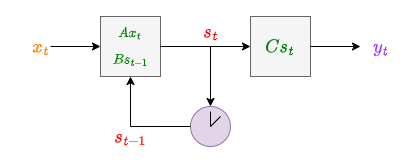
\includegraphics[width=100mm,scale=0.4]{images/rnn_images/lti_diagram.png}
        \end{figure}

        

        This kind of model is often an excellent approximation of simple systems in physics, signals, and other sciences.

        \subsecdiv

        In the next section, we'll add non-linear units to this linear model, and this will create a \vocab{Recurrent Neural Network}.\\



\pagebreak
\fi

\section{Recurrent Neural Networks}

    We've fully fleshed out our state machines above: we've developed a technique for managing time, using \purp{memory}.

    \begin{itemize}
        \item This is similar to how, in the last chapter, we developed Convolution, to manage \gren{space}.
    \end{itemize}

    Just as we did in convolution, we'll add state machines into our neural network system. This will give us the \vocab{Recurrent Neural Network (RNN)}.



    \phantom{}

    \subsection{Building up RNNs}

        How do we create a "network" using our state machine system?

        \begin{itemize}
            \item  Well, a traditional NN applies a \purp{linear} operation $z=W^Tx+W_0$, and then a \purp{non-linear} operation, $a=f(z)$.
            
            \item We'll implement this process in our state machine, using $\grn{f_s}$ and $\grn{f_o}$.
        \end{itemize}

        The \vocab{linear time-invariant (LTI) system} we defined at the end of the last section gives us the simplest, most reduced version of this:

        \begin{equation*}
            \grn{f_s}(\red{s_{t-1}},\bru{x_t}) 
            \;\;=\;\; A\red{s_{t-1}} + B\bru{x_t}
            \qquad \qquad
            \grn{f_o}(\red{s_t}) 
            \;\;=\;\; C\red{s_t}
        \end{equation*}

        To replicate a neural network, we'll need to add two things.\\

        \begin{concept}
            An RNN modifies an LTI system in two ways:
    
            \begin{itemize}
                \item Includes \gren{offset} terms in the linear part of $\grn{f_o}$ and $\grn{f_s}$
                \item Adds a \purp{nonlinear} component after the linear component both functions.
            \end{itemize}
        \end{concept}




    \phantom{}

    \subsection{Offset}

        Let's add that offset term:

        \begin{equation*}
            \grn{f_s}(\red{s_{t-1}},\bru{x_t}) 
            \;\;=\;\; As_{t-1} + Bx_t + \blu{D}
            \qquad \qquad
            \grn{f_o}(\red{s_t}) 
            \;\;=\;\; Cs_t + \blu{E}
        \end{equation*}

        This is a bit cluttered. We'll rename all of these weights:\\

        \begin{notation}
            For our RNN, we'll label our \vocab{weights} as $W^{ab}$:

            \begin{itemize}
                \item $b$ represents the "\pink{input}": what we're multiplying $W^{ab}$ with.
                \item $a$ represents the "\brun{output}": what we're using $W^{ab}$ to compute.
            \end{itemize}

            We'll also use subscript $W_0$ for offset terms.
            
        \end{notation}

        We can go through all of our weights like this.\\

        \begin{notation}
            We want to rewrite $\grn{f_s}(\red{s_{t-1}},\bru{x_t}) 
            \;\;=\;\; As_{t-1} + Bx_t + \blu{D}$
            
            \begin{itemize}
                \item $W^{ss}$ is combined with $s_{t-1}$, to compute $s_t$.
                \item $W^{sx}$ is combined with $x_t$, to compute $s_t$.
                \item $W^{ss}_0$ is the offset term that computes $s_t$.
            \end{itemize}

            \begin{equation*}
                s_t = W^{ss}\red{s_{t-1}} + W^{sx}\bru{x_t} + \blu{W^{ss}_0}
            \end{equation*}

            Now, we'll rewrite $\grn{f_o}(\red{s_t}) 
            \;\;=\;\; Cs_t + \blu{E}$:

            \begin{itemize}
                \item $W^{o}$ is combined with $s_t$ to compute the $y_t$. 
                
                \begin{itemize}
                    \item Based on conventions, you could also write it as $W^{os}$. But, since there's no $x$ term, this is unnecessary.
                \end{itemize}

                \item $W^o_0$ is the offset term that computes $y_t$.
            \end{itemize}

            \begin{equation*}
                y_t = W^o\red{s_t} + \blu{W^o_0}
            \end{equation*}
        \end{notation}

        \begin{figure}[H]
            \centering
            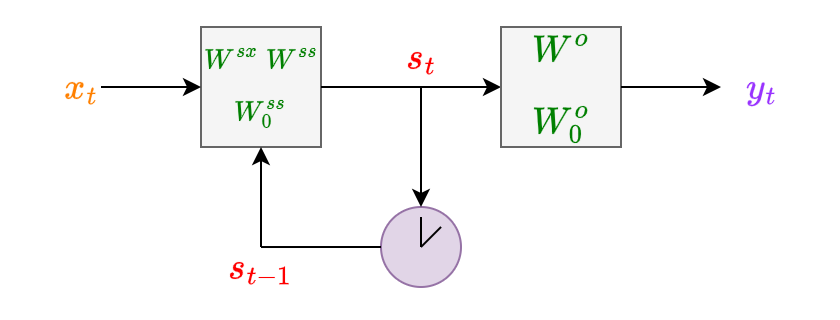
\includegraphics[width=100mm,scale=0.4]{images/rnn_images/rnn_diagram_linear.png}
        \end{figure}



    \phantom{}

    \subsection{Activation Function}

        Now, we've covered the linear part of our function. We'll apply a non-linear function $f$ and $g$ to each:

        \begin{equation}
            s_t = \grn{f} \Big( W^{ss}\red{s_{t-1}} + W^{sx}\bru{x_t} + \blu{W^{ss}_0} \Big)
        \end{equation}

        \begin{equation}
            y_t = \grn{g} \Big( W^o\red{s_t} + \blu{W^o_0} \Big)
        \end{equation}

        These are our \purp{activation functions}.

        $f$ and $g$ are pretty vague names, so it would be more helpful to name them according to what they're being used to compute: state and output.

        \begin{itemize}
            \item So, we could say $f=f_s$, and $g=f_o$.\\
        \end{itemize}

        \begin{clarification}
            In previous sections, we've used \grn{$f_s$} and \grn{$f_o$} to indicate the \orgg{entire function} used to compute the state/output, including the \purp{linear} part.

            \begin{itemize}
                \item However, we want to separate the linear and \gren{non-linear} parts.
            \end{itemize}

            \subsecdiv

            So, we'll switch conventions: $f_s$ and $f_o$ in sections 10.1 and 10.2 are \redd{not the same}.

            \begin{itemize}
                \item $f_s$ and $f_o$ now represent these \gren{activation functions}.
             \end{itemize}
        \end{clarification}

        \begin{equation}
            s_t = \grn{f_s} \Big( W^{ss}\red{s_{t-1}} + W^{sx}\bru{x_t} + \blu{W^{ss}_0} \Big)
        \end{equation}

        \begin{equation}
            y_t = \grn{f_o} \Big( W^o\red{s_t} + \blu{W^o_0} \Big)
        \end{equation}

        We'll insert these units into our diagram:

        \begin{figure}[H]
            \centering
            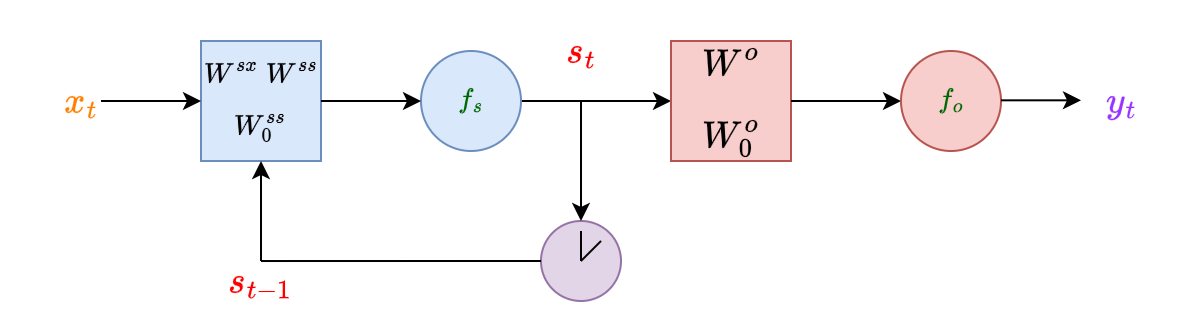
\includegraphics[width=150mm,scale=0.4]{images/rnn_images/rnn_flat.png}
        \end{figure}

        \begin{concept}
            Just like in a traditional neural network, we apply our activation functions \purp{element-wise}.

            \begin{equation*}
                f \left( 
                \begin{bmatrix}
                    a_1 \\ a_2 \\ a_3
                \end{bmatrix}
                \right) 
                =
                \begin{bmatrix}
                    f(a_1) \\ f(a_2) \\ f(a_3)
                \end{bmatrix}
            \end{equation*}
        \end{concept}


    \phantom{}

    \subsection{Shape}

        We've the mechanics of our RNN sorted out. To do some quick book-keeping, we'll address the shapes of our various objects.

        We'll keep our input, state, and output as vectors:\\

        \begin{definition}
            We define the dimensions of our input, output, and state as vectors:

            \begin{equation*}
                \begin{matrix}
                    \bru{\mathcal{X}} = \RR^\ell \\
                    \red{\mathcal{S}} = \RR^m    \\
                    \pur{\mathcal{Y}} = \RR^n
                \end{matrix}
                \qquad\implies\qquad 
                \begin{matrix}
                    \bru{x_t} &:& (\ell \cross 1) \\
                    \red{s_t} &:& (m \cross 1)    \\
                    \pur{y_t} &:& (n \cross 1)
                \end{matrix}
            \end{equation*} 
        \end{definition}

        Based on these vectors, we can derive our weight dimensions:\\

        \begin{definition}
            We define the dimensions of our RNN weights:

            \begin{equation*}
                \begin{matrix}
                    \red{W^{sx}} &:& (m \times \ell) \\
                    \red{W^{ss}} &:& (m \times m) \\
                    \red{W^{ss}_0} &:& (m \times 1) \\
                    \pur{W^{o}} &:& (n \times m)\\
                    \pur{W^{o}_0} &:& (n \times 1)
                \end{matrix}
            \end{equation*} 
        \end{definition}



    \pagebreak

    \subsection{Complete RNN}

        Now, we've done all the work we need to: We can define our RNN.\\

        \begin{definition}
            A \vocab{Recurrent Neural Network (RNN)} is a particular kind of \gren{state machine} used as a neural network:

            \begin{itemize}
                \item We use a state machine so our network can remember and use past data, via the \redd{state}.
                \item We call it "\purp{recurrent}" because of our states. A state is created by the network to find the output, and then one timestep later, is \purp{re-used} as a new input.
            \end{itemize}

            \phantom{}

            Our RNN manipulates input $\bru{x_t \in \RR^\ell}$, and state $\red{s_t \in \RR^m}$, to create an output $\pur{y_t \in \RR^n}$.

            Our state and output equations are given as:

            \begin{equation*}
                s_t = \grn{f_s} \Big( W^{ss}\red{s_{t-1}} + W^{sx}\bru{x_t} + \blu{W^{ss}_0} \Big)
            \end{equation*}

            \begin{equation*}
                y_t = \grn{f_o} \Big( W^o\red{s_t} + \blu{W^o_0} \Big)
            \end{equation*}

            Where $f_s$ and $f_o$ are (typically non-linear) \purp{activation functions}, and every weight $W$ is a \gren{matrix} with the appropriate dimensions.
        \end{definition}

        \begin{figure}[H]
            \centering
            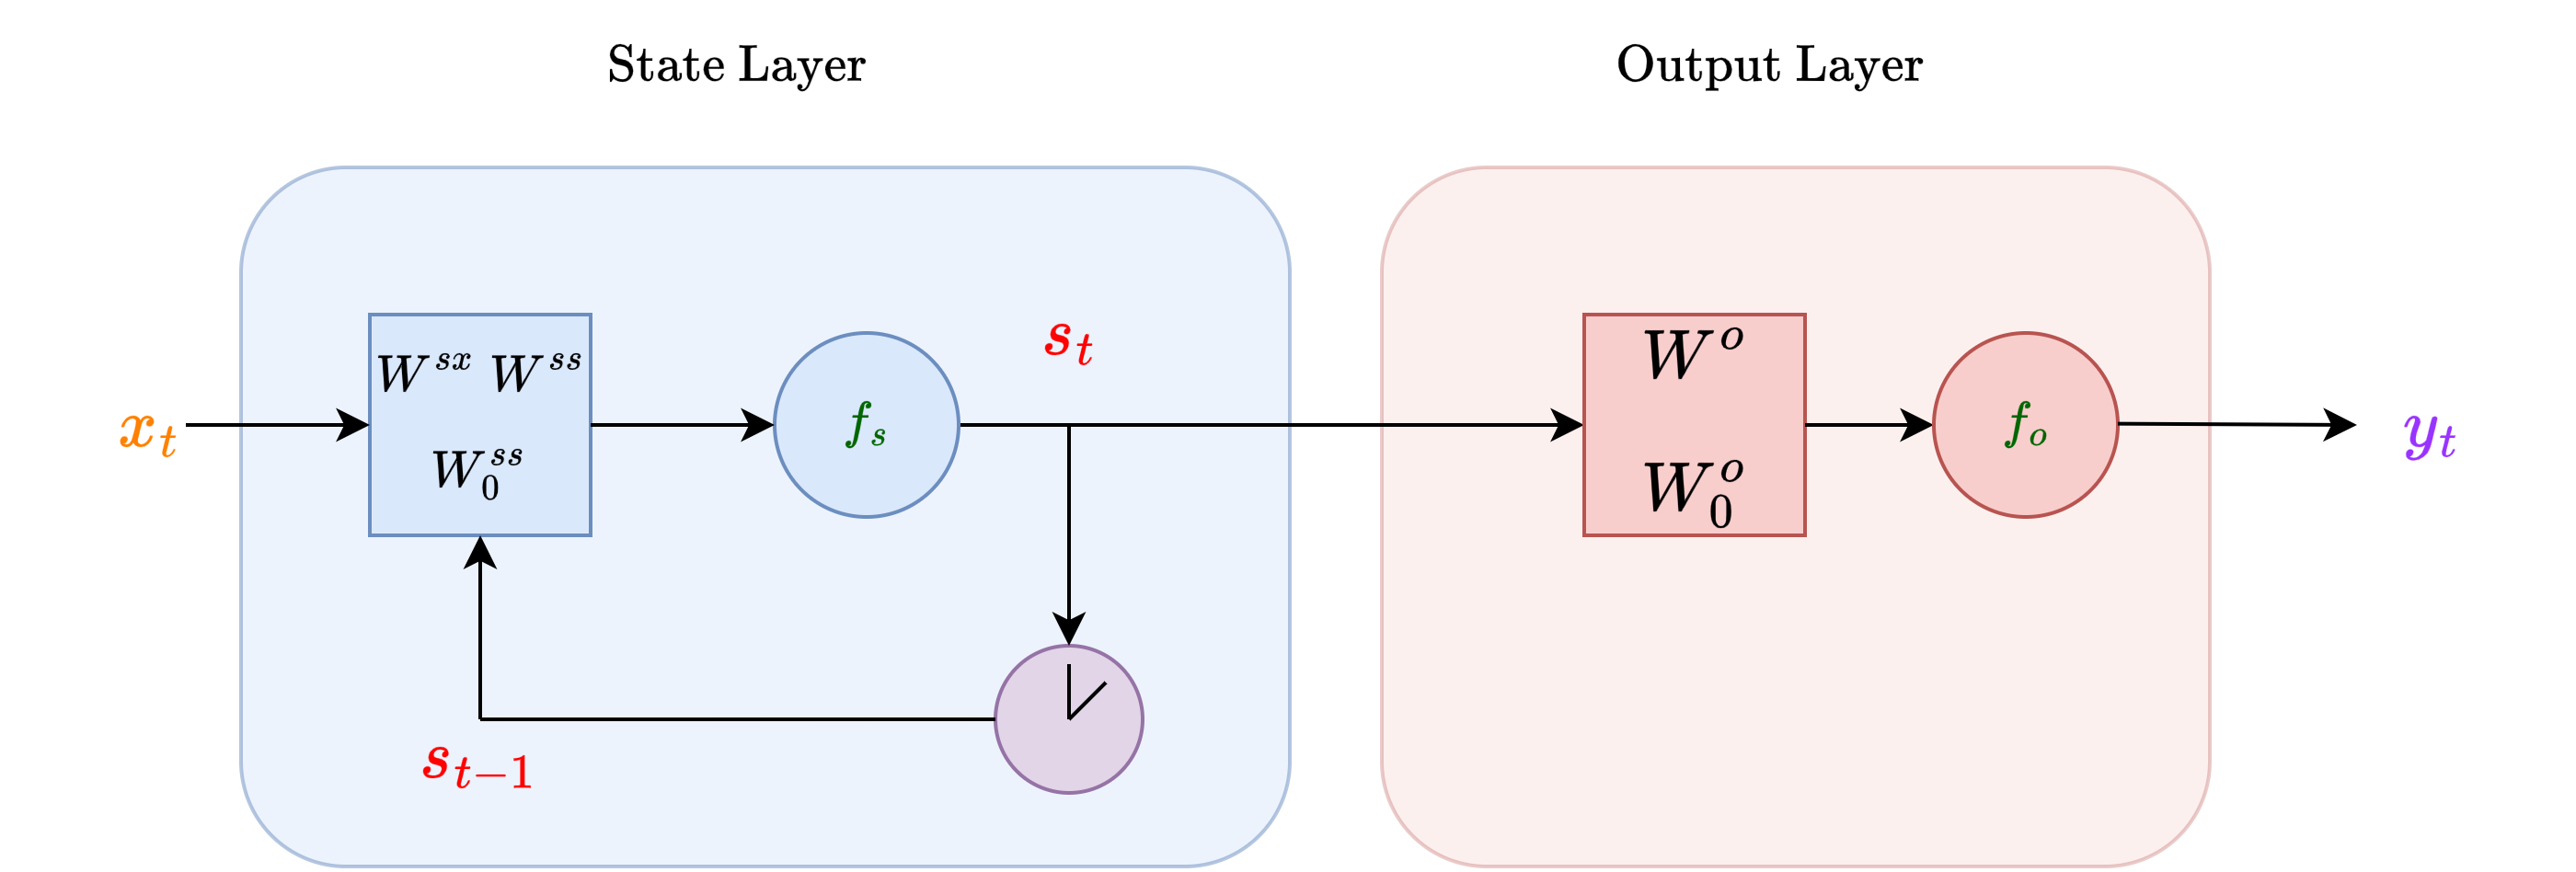
\includegraphics[width=150mm,scale=0.4]{images/rnn_images/rnn_full.png}
        \end{figure}

        We can abstract away all the math with a simpler perspective:
            \note{Technically, this diagram works for any state machine.}

        \begin{figure}[H]
            \centering
            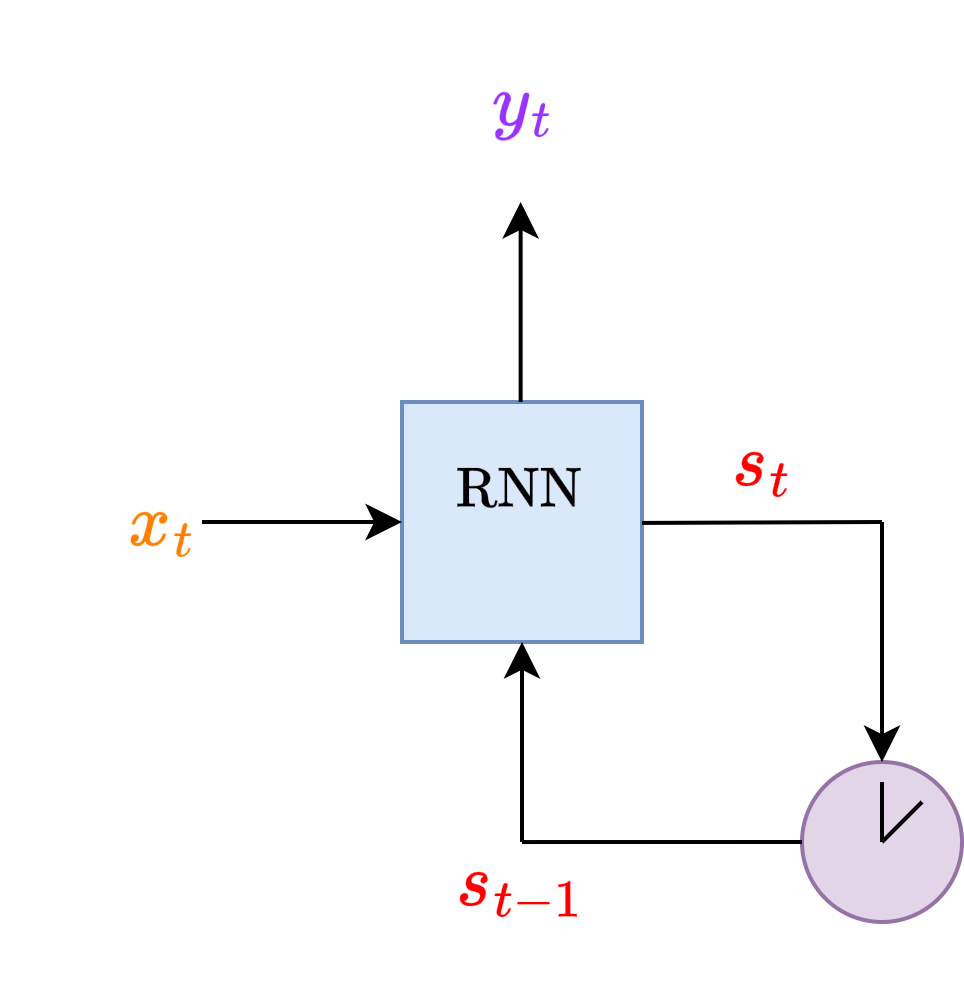
\includegraphics[width=50mm,scale=0.4]{images/rnn_images/simplified_rnn.png}
            \caption*{We have the basic parts we care about: input, output, and state. 
            
            Our input and output are visible from outside, while the \redd{state} is recycled within the system. }
        \end{figure}

        Take a moment to compare this model to the more complex one above: they're more similar than they seem.


    \phantom{}

    \subsection{RNN as a "network"}

        One issue we might have with the above diagram is it doesn't look very much like a \purp{network}: at best, it seems like a very small network.

        But the simplified diagram could inspire us: currently, the RNN "feeds into itself", using the state. 

        \begin{itemize}
            \item In a different perspective, we could imagine that our first RNN unit is feeding into a second, \gren{identical} unit.
            \item We'll show what we mean, by removing the clock:
        \end{itemize}

        \begin{figure}[H]
            \centering
            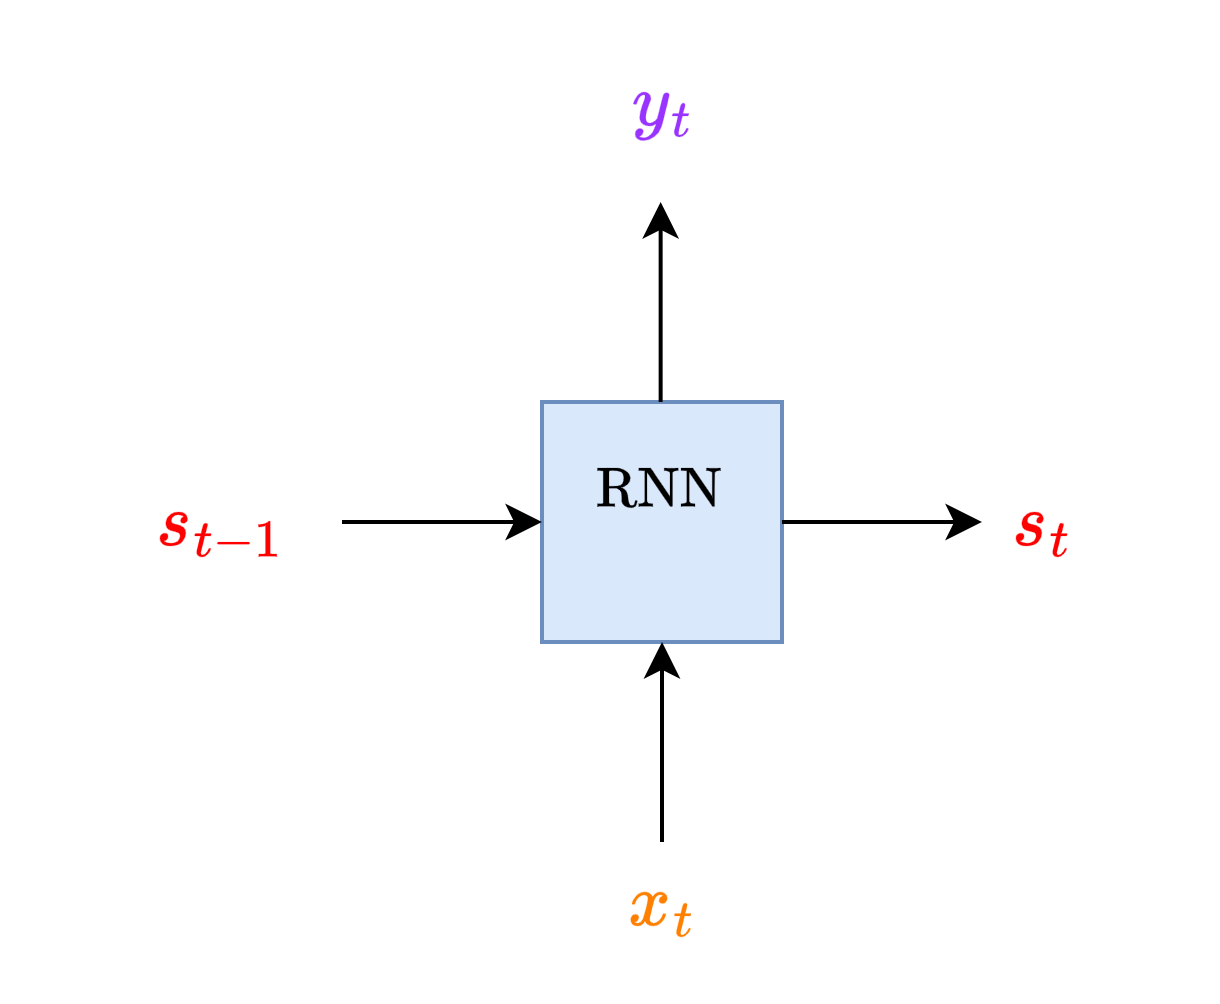
\includegraphics[width=50mm,scale=0.4]{images/rnn_images/noclock_rnn.png}
            \caption*{We have an isolated, simple block.}
        \end{figure}

        Now, we can connect several of these in \orgg{series}: each one represents the input and output for the $\nth{t}$ timestep. 

        \begin{itemize}
            \item The state $s_t$ feeds into the $\nth{(t+1)}$ block.
        \end{itemize}

        \begin{figure}[H]
            \centering
            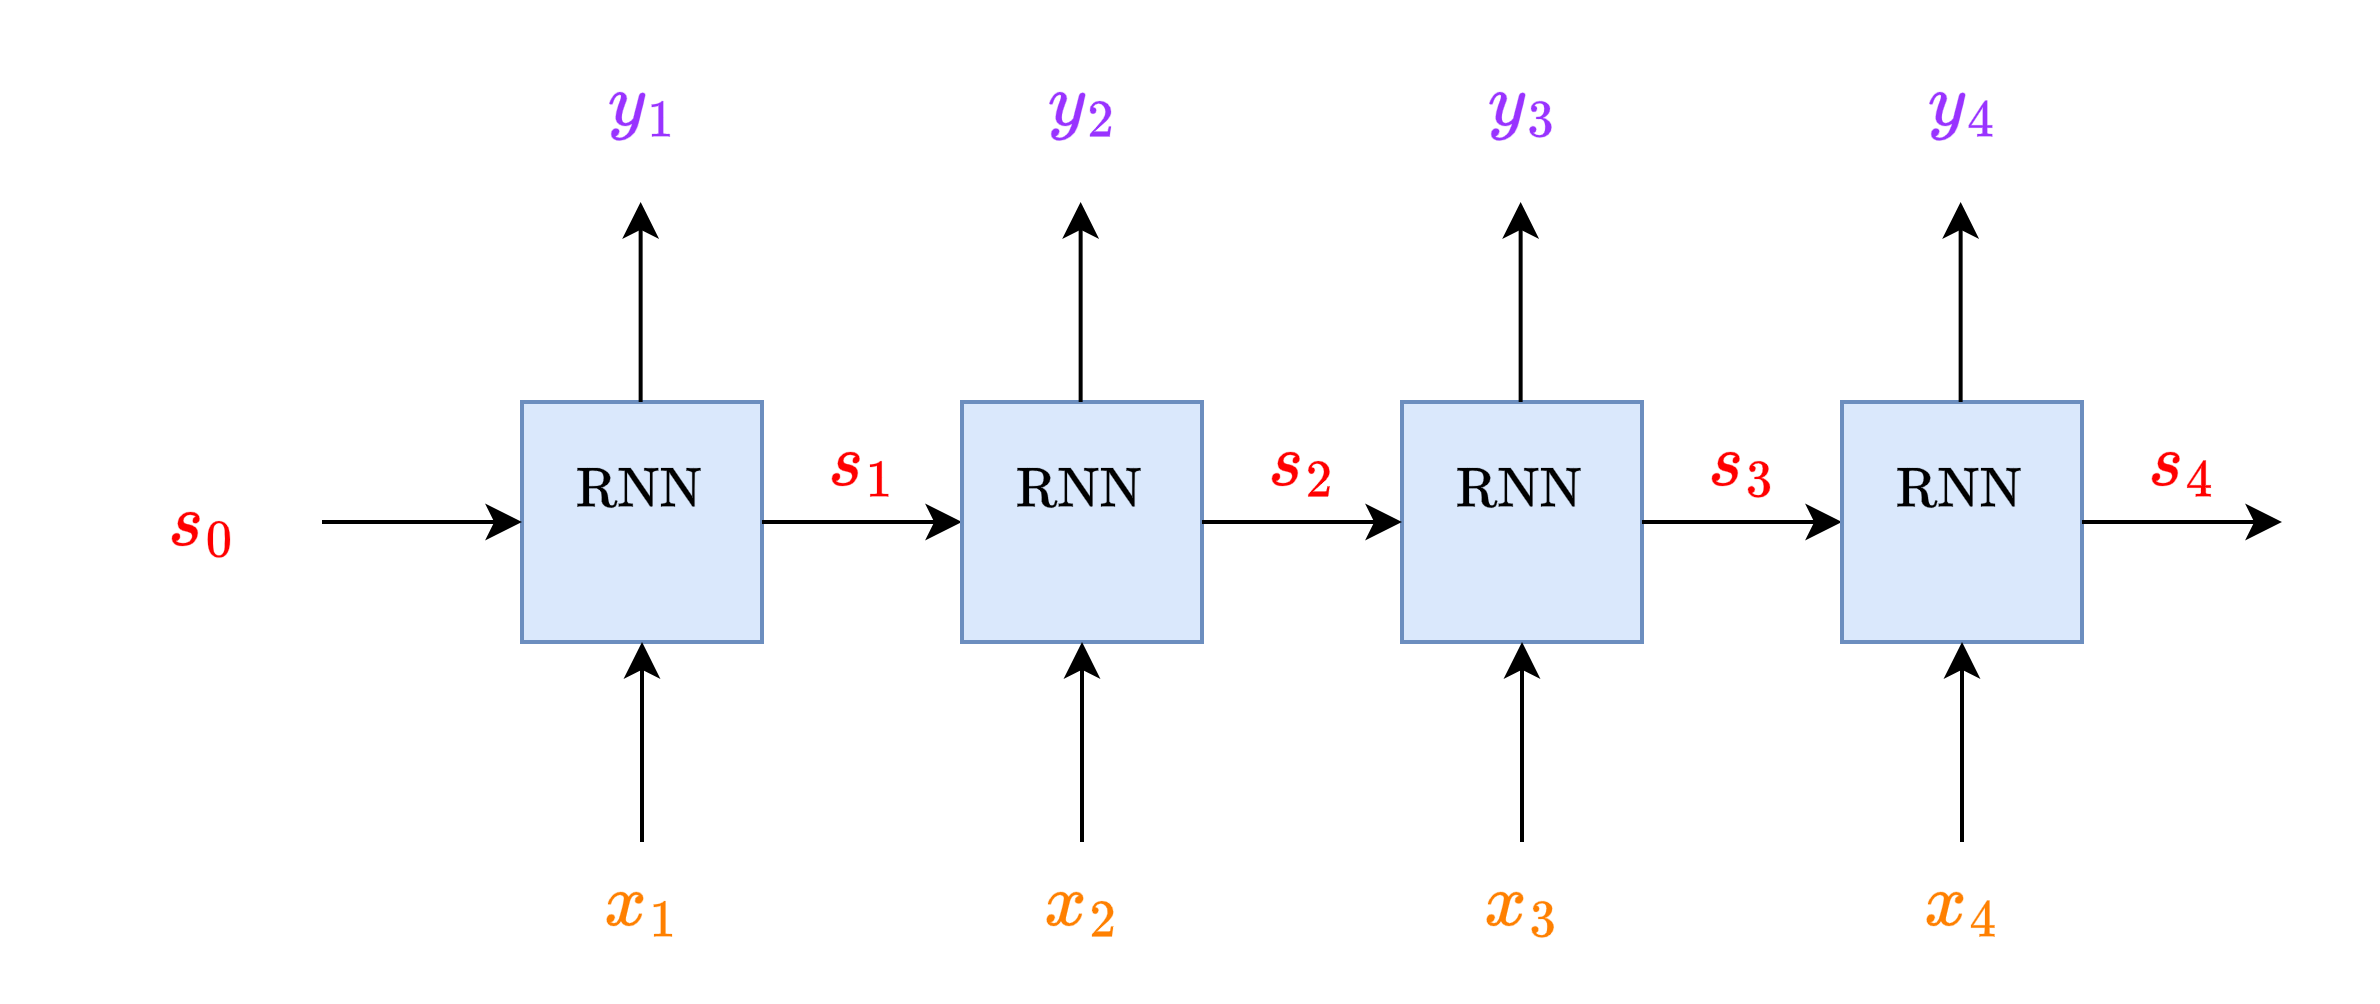
\includegraphics[width=150mm]{images/rnn_images/rnn_simple_layers.png}
            \caption*{Each of these RNNs is the same block: we've replaced our loop by copying the same RNN multiple times.}
        \end{figure}

        Now, it looks more like a network! This is fascinating: an RNN is like a network where we use the \gren{same layer} over and over again!

        \begin{itemize}
            \item With the additional caveat that each layer has its own \redd{input} and \gren{output}.\\
        \end{itemize}

        \begin{concept}
            One perspective on RNNs is to see them as a \orgg{layered} network, where each layer is the full RNN:

            \begin{itemize}
                \item Every layer has a \purp{distinct} input and an output.
                \item Every layer is structurally \gren{identical} (same weights, activation).
            \end{itemize}
        \end{concept}

        Of course, this version can be misleading: we don't actually have $n$ copies of our RNN, we have one copy that we're using repeatedly.

        \begin{itemize}
            \item However, we could think of the $x$-axis as representing "time": the same RNN reused at multiple times.
        \end{itemize}




    \phantom{}

    \subsection{RNN fully unpacked}

        Now that we've introduced this perspective, let's use it for the "\orgg{unpacked}" version of our RNN, where we don't hide all of our inner functions. This will get a little messy.

        First, we need to remove the clock:

        \begin{figure}[H]
          \centering
          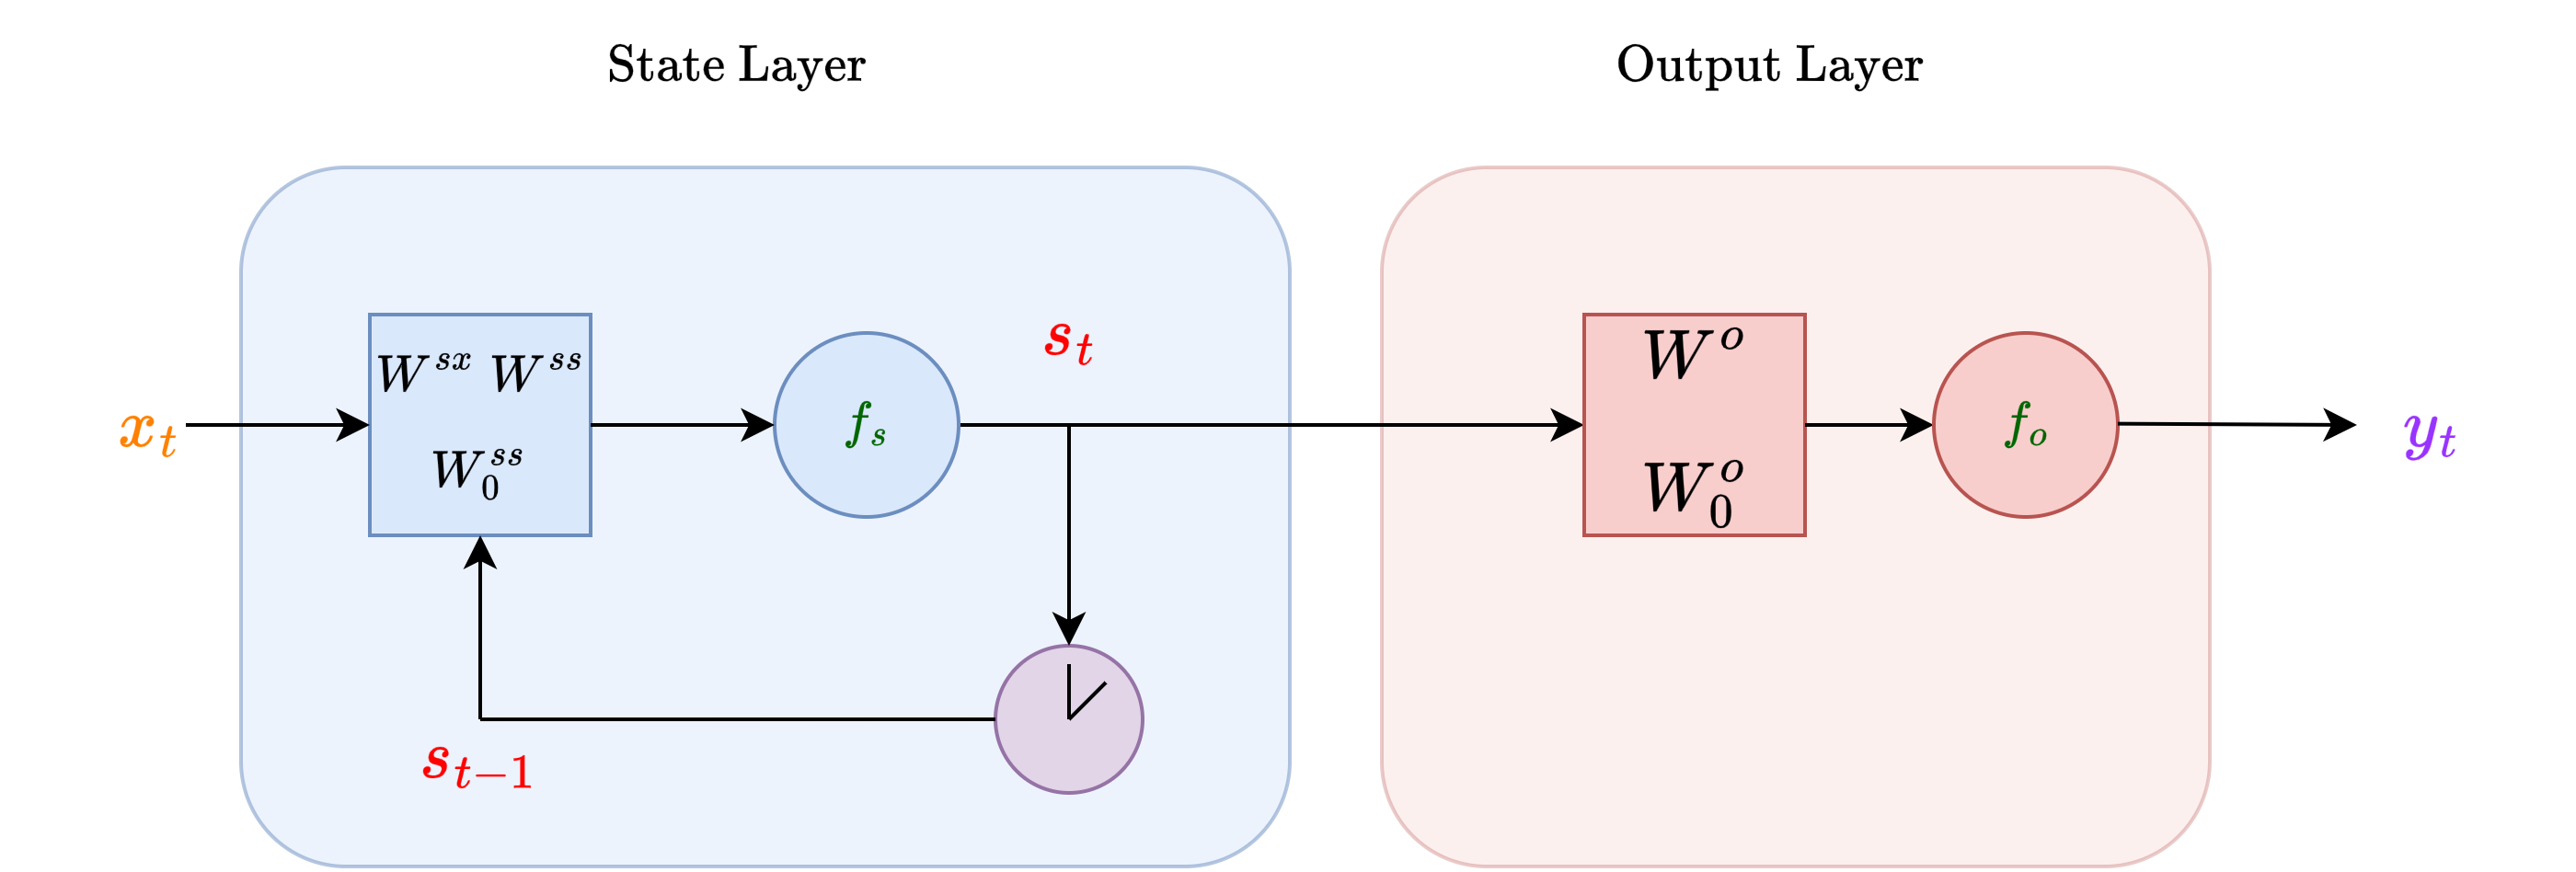
\includegraphics[width=\linewidth]{images/rnn_images/rnn_full.png}
          \caption*{Our RNN, unpacked.}
        \end{figure}

        \begin{figure}[H]
          \centering
          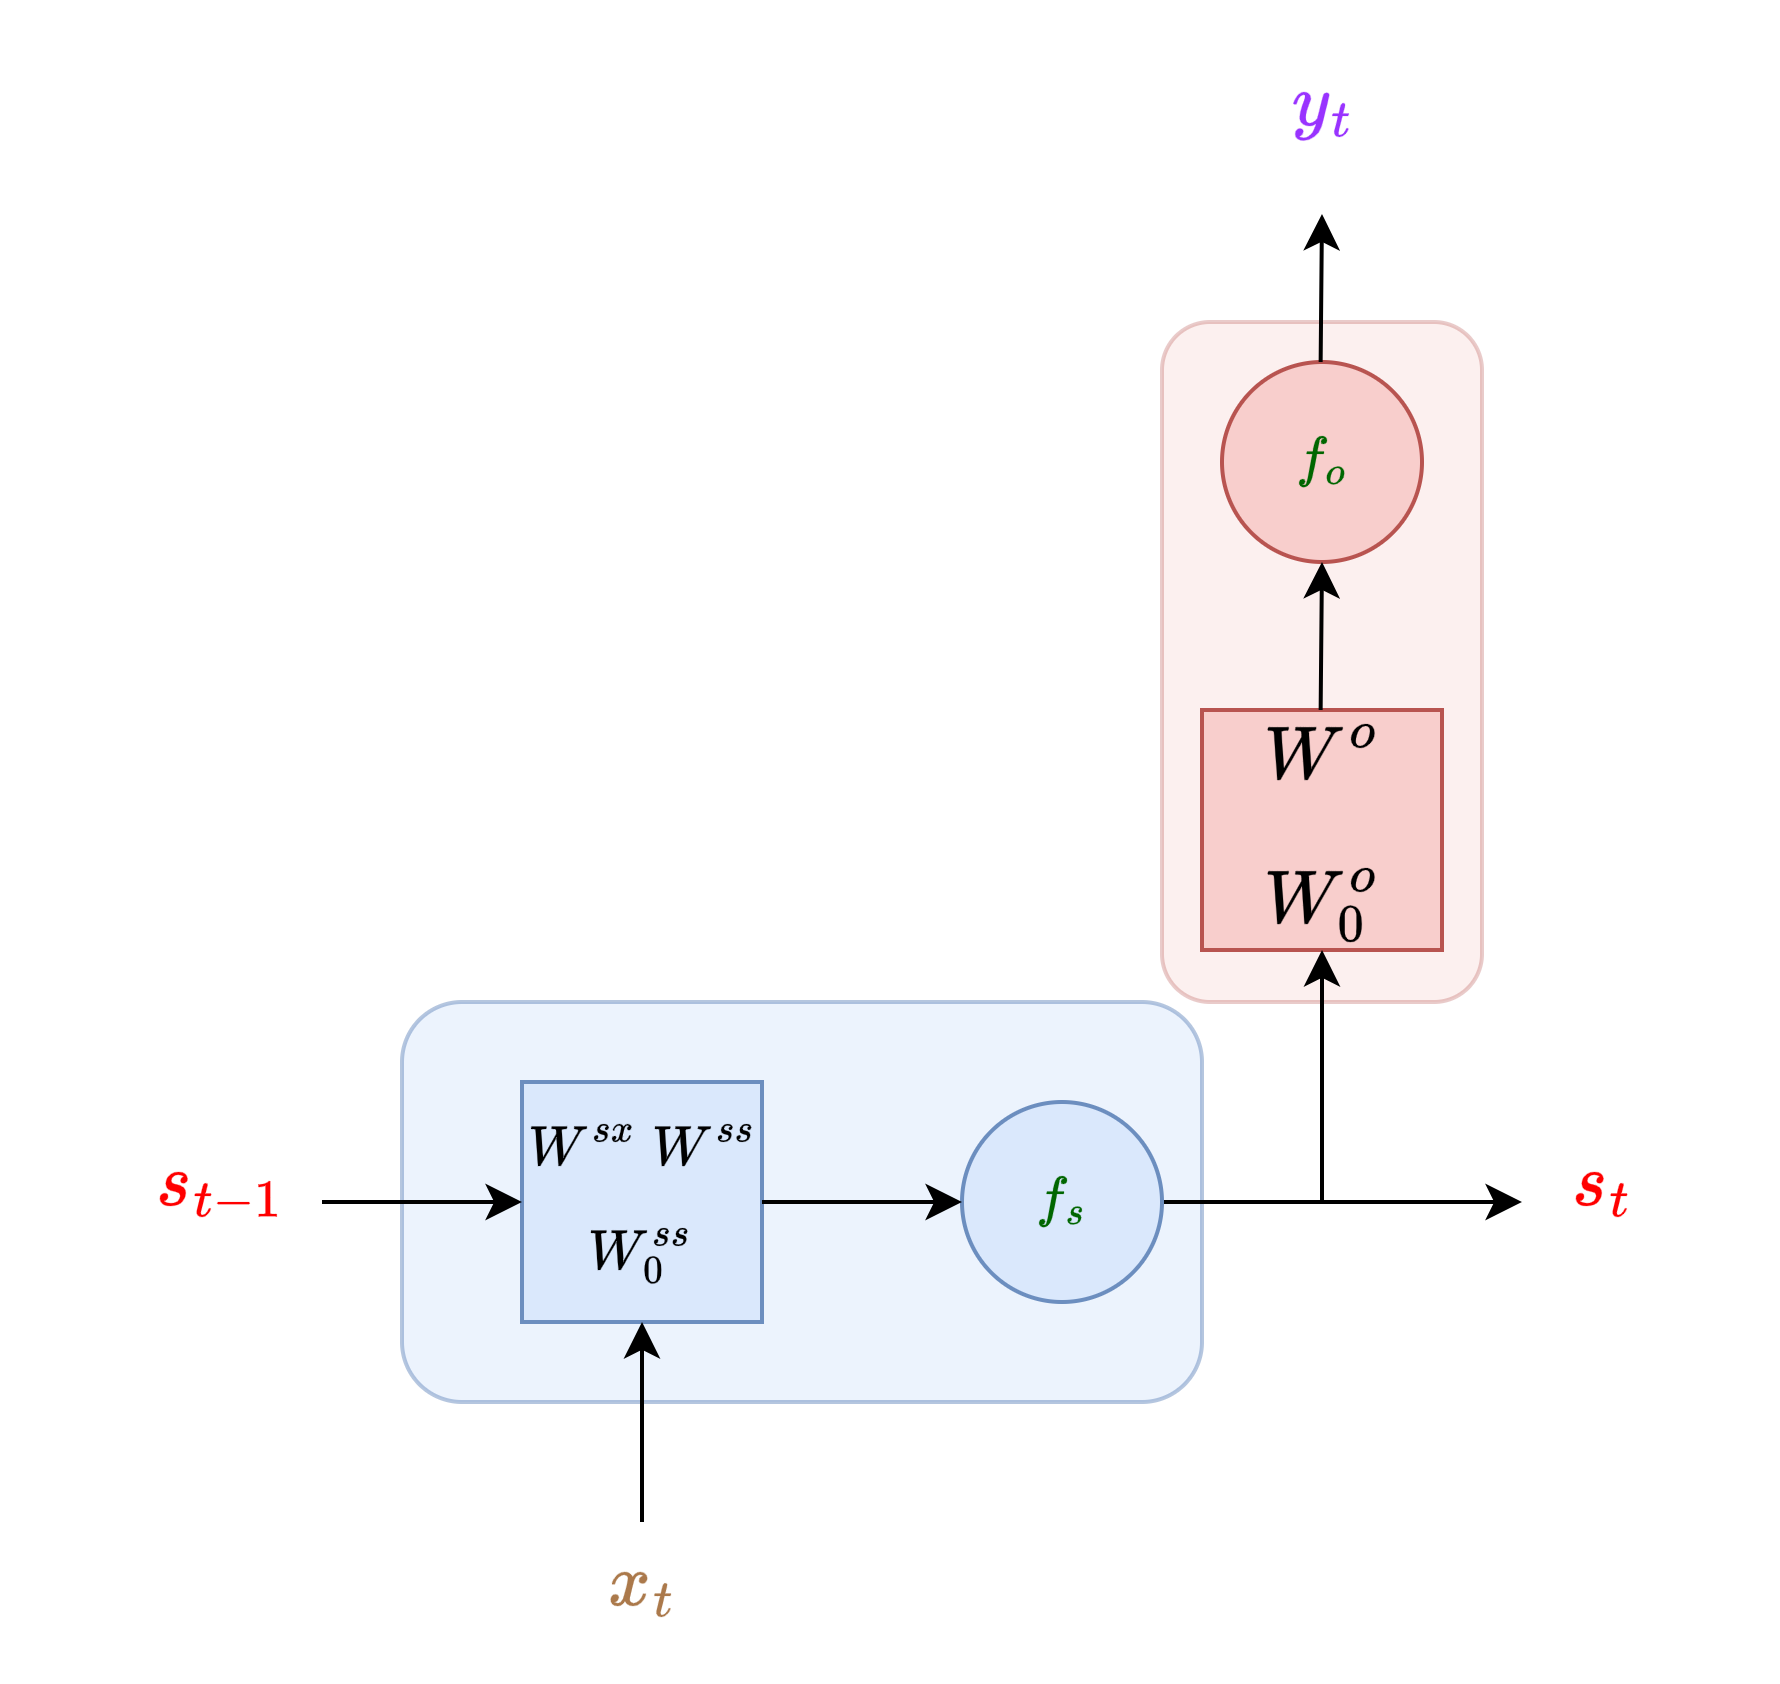
\includegraphics[width=.5\linewidth]{images/rnn_images/unrolled_rnn.png}
          \caption*{Our RNN, clock removed.}
        \end{figure}

        We had to rearrange things a bit to get the effect we wanted.

        But now, we can stack these into a full "network":

        \begin{figure}[H]
          \centering
          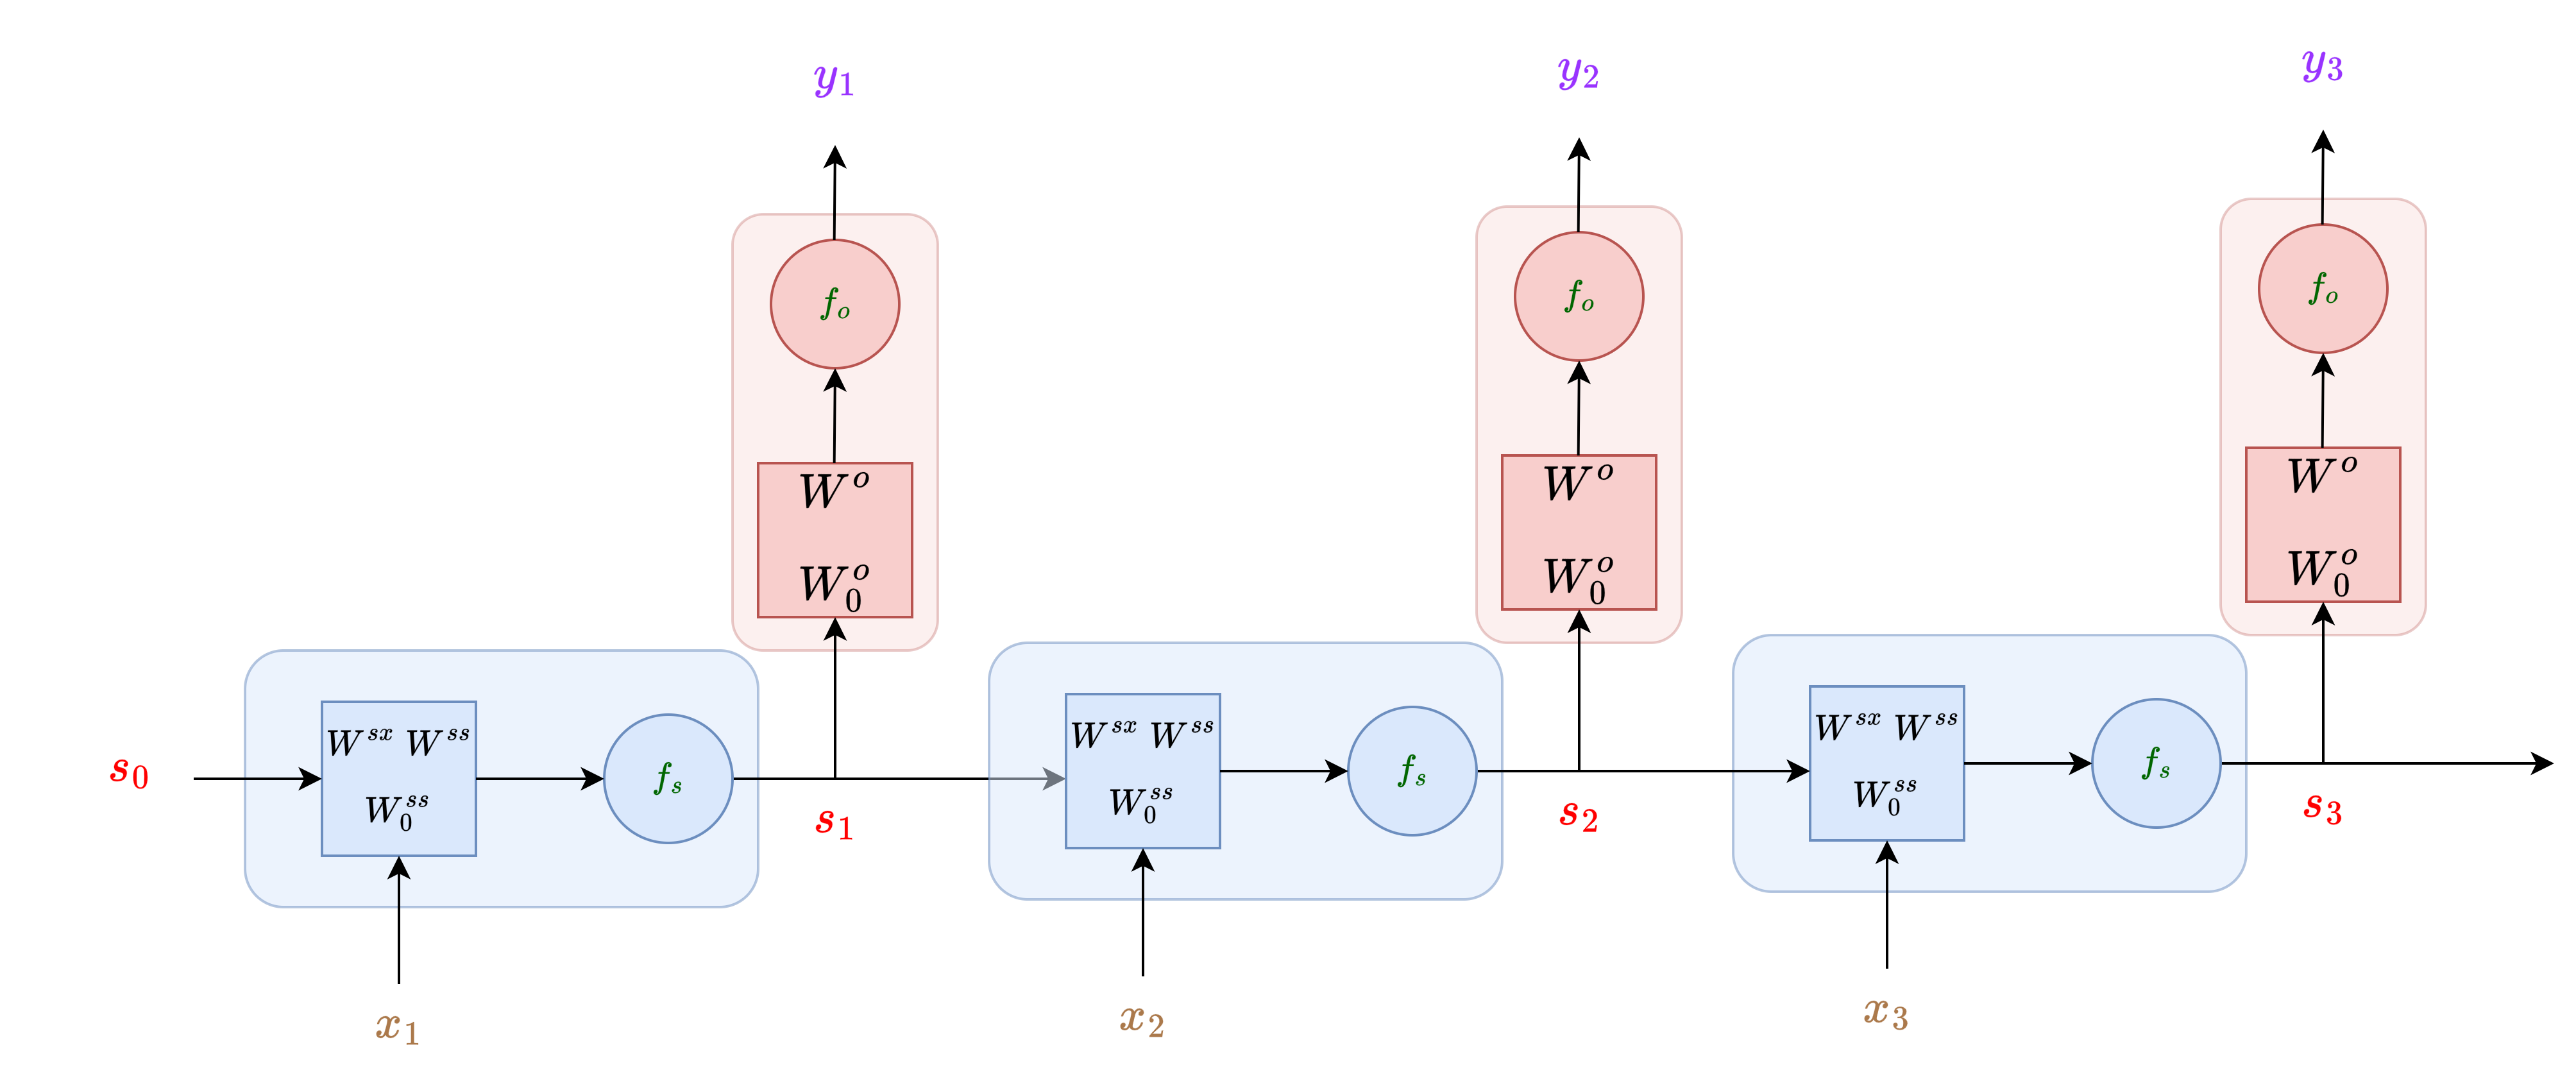
\includegraphics[width=\linewidth]{images/rnn_images/multilayer_unrolled_rnn.png}
          \caption*{Our RNN, unpacked.}
        \end{figure}

        This version looks complex, but it's just three copies of our previous model, side-by-side.


    \pagebreak 

    \subsection{RNN Example 1 (\redd{Optional})}

        Let's try a very simple example: we'll do a \orgg{weighted average} of the last 3 inputs.

        This is a linear operation, so we can ignore the activation functions. Thus, $\grn{f_s}$ and $\grn{f_o}$ are the identity function: $\grn{f_s}(z)=\grn{f_o}(z)=z$

        \begin{equation}
            s_t = W^{ss}\red{s_{t-1}} + W^{sx}\bru{x_t} + \blu{W^{ss}_0}
        \end{equation}

        \begin{equation}
            y_t = W^o\red{s_t} + \blu{W^o_0} 
        \end{equation}

        Our input $x_t$ for each turn will be a single value, stored in a $(1 \times 1)$ matrix. Likewise, the "weighted average of 3 inputs" is a single value: another $(1 \times 1)$.

        \begin{equation}
            x_t = \begin{bmatrix}
                X_t
            \end{bmatrix}
            \qquad \qquad
            y_t = \begin{bmatrix}
                Y_t
            \end{bmatrix}
        \end{equation}

        \begin{itemize}
            \item Our state is based on the information we need to remember in order to compute the output.
            \item Thus, we'll store the \purp{last three inputs}.
        \end{itemize}

        \begin{equation}
            s_t = \begin{bmatrix}
                X_{t-2} \\ X_{t-1} \\ X_{t}
            \end{bmatrix}
        \end{equation}

        \begin{concept}
            Our \vocab{state vector} is typically chosen based on what is useful for finding the \purp{output}. 
        \end{concept}

        \subsecdiv

        So, our goal is to get the structure we gave $s_t$ above. We'll need to encode that in our equation.

        We compute $s_t$ from $s_{t-1}$, $x_t$, and an offset.

        \begin{itemize}
            \item We're storing our past values, so we don't need an offset: $W_o^{ss}=0$.
        \end{itemize}

        \begin{equation}
            \begin{bmatrix}
                X_{t-2} \\ X_{t-1} \\ X_{t}
            \end{bmatrix} 
            = W^{ss}\red{s_{t-1}} + W^{sx}\bru{x_t}
            \quad \implies \quad
            \begin{bmatrix}
                \blu{X_{t-2}} \\ \blu{X_{t-1}} \\ \blu{X_{t}}
            \end{bmatrix}
            =
            W^{ss}\begin{bmatrix}
                X_{t-3} \\ \red{X_{t-2}} \\ \red{X_{t-1}}
            \end{bmatrix} 
            + 
            W^{sx}
            \begin{bmatrix}
                \bro{X_t}
            \end{bmatrix}
        \end{equation}

        Now, we can see that the information for $s_t$ is spread across both terms:

        \begin{itemize}
            \item The \red{$s_{t-1}$} term contains \red{$X_{t-1}$} and \red{$X_{t-2}$}
            \item The \bro{$x_t$} term contains \bro{$X_t$}. 
        \end{itemize}

        So, we want to end up with:

        \begin{equation}
            \begin{bmatrix}
                \blu{X_{t-2}} \\ \blu{X_{t-1}} \\ \blu{X_{t}}
            \end{bmatrix} 
            =
            \overbrace{
                \begin{bmatrix}
                    \red{X_{t-2}} \\ \red{X_{t-1}} \\ 0
                \end{bmatrix}
            }^{W^{ss}\red{s_{t-1}} }
            +
            \overbrace{
                \begin{bmatrix}
                    0 \\ 0 \\ \bro{X_t}
                \end{bmatrix}
            }^{W^{sx}\bru{x_t}}
        \end{equation}

    \subsecdiv

        We can figure out our weight matrices $W^{ss}$ and $W^{sx}$, by comparing our input and output.
            \note{For starters, we showed above that the dimensions of $W^{sx}$ depend on $x_t$ and $s_t$.}


        \begin{equation}
            \overbrace{
                \begin{bmatrix}
                    ? & ? & ? \\
                    ? & ? & ? \\
                    ? & ? & ?
                \end{bmatrix}
            }^{W^{ss}}
            \begin{bmatrix}
                X_{t-3} \\ \red{X_{t-2}} \\ \red{X_{t-1}}
            \end{bmatrix} 
            = 
            \begin{bmatrix}
                \red{X_{t-2}} \\ \red{X_{t-1}} \\ 0
            \end{bmatrix}
        \end{equation}

        To figure out $W_{ss}$, we go row-by-row, and figure out the correct values:

        \begin{equation}
            \overbrace{
                \begin{bmatrix}
                    \grn{a} & \grn{b} & \grn{c} \\
                    ? & ? & ? \\
                    ? & ? & ?
                \end{bmatrix}
            }^{W^{ss}}
            \begin{bmatrix}
                X_{t-3} \\ \red{X_{t-2}} \\ \red{X_{t-1}}
            \end{bmatrix} 
            = 
            \begin{bmatrix}
                \red{X_{t-2}} \\ \red{X_{t-1}} \\ 0
            \end{bmatrix}
            \quad \implies \quad 
            \grn{a}X_{t-3}+\grn{b}\red{X_{t-2}}+ \grn{c}X_{t-1} = \red{X_{t-2}}
        \end{equation}

        We find $\grn{a}=0$, $\grn{b}=1$, $\grn{c}=0$. We can repeat this process for our other rows.

        Once we do the rest, we find:

        \begin{equation}
            \overbrace{
                \begin{bmatrix}
                    0 & 1 & 0 \\
                    0 & 0 & 1 \\
                    0 & 0 & 0
                \end{bmatrix}
            }^{W^{ss}}
            \begin{bmatrix}
                X_{t-3} \\ \red{X_{t-2}} \\ \red{X_{t-1}}
            \end{bmatrix} 
            = 
            \begin{bmatrix}
                \red{X_{t-2}} \\ \red{X_{t-1}} \\ 0
            \end{bmatrix}
        \end{equation}

        We follow the same logic for the other example:

        \begin{equation}
            \overbrace{
                \begin{bmatrix}
                    0 \\ 0 \\ 1
                \end{bmatrix}
            }^{W^{sx}}
            \begin{bmatrix}
                \bro{X_t}
            \end{bmatrix}
            =
            \begin{bmatrix}
                0 \\ 0 \\ \bro{X_t}
            \end{bmatrix}
        \end{equation}

        \begin{concept}
            In order to derive our weight matrix, we can go \purp{row-by-row}:

            \begin{itemize}
                \item For each row, we figure out which choice of \gren{weights} gives the desired output.
            \end{itemize}
        \end{concept}

        Taken together, we get:

        \begin{equation}
            \begin{bmatrix}
                \blu{X_{t-2}} \\ \blu{X_{t-1}} \\ \blu{X_{t}}
            \end{bmatrix}
            =
            \overbrace{
                \begin{bmatrix}
                    0 & 1 & 0 \\
                    0 & 0 & 1 \\
                    0 & 0 & 0
                \end{bmatrix}
            }^{W^{ss}}
            \begin{bmatrix}
                X_{t-3} \\ \red{X_{t-2}} \\ \red{X_{t-1}}
            \end{bmatrix} 
            + 
            \overbrace{
                \begin{bmatrix}
                    0 \\ 0 \\ 1
                \end{bmatrix}
            }^{W^{sx}}
            \begin{bmatrix}
                \bro{X_t}
            \end{bmatrix}
        \end{equation}

        \subsecdiv

        Now we can compute the weighted average. We'll pick some arbitrary numbers: 50\% of $X_t$, 30\% of $X_{t-1}$, and 20\% of $X_{t-2}$.

        \begin{equation}
            Y_t = 0.5X_t + 0.3X_{t-1} + 0.2X_{t-2}
        \end{equation}

        \begin{itemize}
            \item Again, we don't need an offset $W_0^o=0$.
        \end{itemize}

        \begin{equation}
            \begin{bmatrix}
                Y_t
            \end{bmatrix} = W^o\red{s_t}
            \quad \implies \quad
            W^o 
            \begin{bmatrix}
                \blu{X_{t-2}} \\ \blu{X_{t-1}} \\ \blu{X_{t}}
            \end{bmatrix} 
        \end{equation}

        We can, again, figure out our weight matrix $W^o$ based on the desired result.

        \begin{equation*}
            \overbrace{
                \begin{bmatrix}
                    0.5 & 0.3 & 0.2
                \end{bmatrix}
            }^{W^o}
            \begin{bmatrix}
                \blu{X_{t-2}} \\ \blu{X_{t-1}} \\ \blu{X_{t}}
            \end{bmatrix} 
            =
            0.5X_t + 0.3X_{t-1} + 0.2X_{t-2}
        \end{equation*}

        \begin{remark}
            Our final RNN comes out to:

            \begin{equation*}
                \grn{f_s}(z)=\grn{f_o}(z)=z
            \end{equation*}

            \begin{equation*}
                W^{ss} = \begin{bmatrix}
                    0 & 1 & 0 \\
                    0 & 0 & 1 \\
                    0 & 0 & 0
                \end{bmatrix} \qquad
                W^{sx} = \begin{bmatrix}
                    0 \\ 0 \\ 1
                \end{bmatrix} \qquad
                W^{ss}_0 = \begin{bmatrix}
                    0 \\ 0 \\ 0
                \end{bmatrix}
            \end{equation*}

            \begin{equation*}
                W^{o} = \begin{bmatrix}
                    0.5 & 0.2 & 0.2
                \end{bmatrix} \qquad
                W^{o}_0 =\begin{bmatrix}
                    0
                \end{bmatrix}
            \end{equation*}
        \end{remark}

        

        

        

        

    \pagebreak

    \subsection{RNN Example 2 (\redd{Optional})}

        Let's run through a more concrete example.

        For simplicity, $\grn{f_s}$ and $\grn{f_o}$ are the identity function: $\grn{f_s}(z)=\grn{f_o}(z)=z$.
            \note{Remember that this is the activation function, not the complete function we use}

        \begin{equation}
            s_t = W^{ss}\red{s_{t-1}} + W^{sx}\bru{x_t} + \blu{W^{ss}_0}
        \end{equation}

        \begin{equation}
            y_t = W^o\red{s_t} + \blu{W^o_0} 
        \end{equation}

        \subsecdiv

        \begin{itemize}
            \item Each \brun{input} is one number: the amount of money you earn every month.

            \begin{equation}
                x_t = \begin{bmatrix}
                    \bro{x^{E}_t}
                \end{bmatrix}
            \end{equation}
            \item Our \redd{state} will be two numbers: the money you have in the bank, and the money you've invested.

            \begin{equation}
                s_t = \begin{bmatrix}
                    \red{s^{B}_t} \\ \red{s^{I}_t}
                \end{bmatrix}
            \end{equation}

            \item Your \purp{output} is your net worth: including the bank, and the invested money.

            \begin{equation}
                y_t = \begin{bmatrix}
                    \pur{y^{T}_t}
                \end{bmatrix}
            \end{equation}
        \end{itemize}

        Each of these could be a vector of any length, depending on the problem.

        \subsecdiv

        First, we want to compute $s_t$. Just like we mentioned in \vocab{Example 1}, we can go row-by-row to figure out the equation for $s_t$.
        
        Let's starting with your first row, $s_t^{B}$: your "savings" money.

        \begin{itemize}
            
            \item The money in the bank $\red{s^{B}_{t-1}}$ makes no interest. 
                \note{We have a pretty terrible bank.}
            \item 10\% of our investing $\red{s^{I}_{t-1}}$ goes into the bank.
            \item 80\% of our earned money $\bro{x_{t}^{E}}$ goes into the bank.
            \item We lose \blu{\$6000} of savings every month.

            \begin{equation}
                s_t^{B} =  \red{s^{B}_{t-1}} + 0.2\red{s^{I}_{t-1}} + 0.8\bro{x_{t}^{E}} - \blu{6000}
            \end{equation}
            
        \end{itemize}

        With this, we can write in vector form:

        \begin{equation}
            \begin{bmatrix}s_t^{B}\end{bmatrix} = 
            \begin{bmatrix}
                1 & 0.2
            \end{bmatrix}
            \begin{bmatrix}
                \red{s^{B}_{t-1}} \\ \red{s^{I}_{t-1}}
            \end{bmatrix}
            +
            \begin{bmatrix}0.8\end{bmatrix}
            \begin{bmatrix}\bro{x_{t}^{E}}\end{bmatrix}
            - \blu{6000}
        \end{equation}

        \begin{concept}
            Just like in other neural networks, the \gren{weights} in an RNN indicate how an \redd{input} variable (ex: $x_t^E$) affects an \purp{output} variable (ex: $s_t^B$ in our linear system)
        \end{concept}

        \subsecdiv

        Now, we'll compute $s_t^I$, your investment money:

        \begin{itemize}
            \item The money in the bank $\red{s^{B}_{t-1}}$ is not invested.
            \item Our invested money $\red{s^{I}_{t-1}}$ grows by 1\%.
            \item 20\% of our earned money $\bro{x_{t}^{E}}$ is invested.
            \item \blu{No money} is added beyond that.
        \end{itemize}

        \begin{equation}
            s_t^{I} =  0\red{s^{B}_{t-1}} + 1.01\red{s^{I}_{t-1}} + 0.2\bro{x_{t}^{E}} + \blu{0}
        \end{equation}

        In vector form:\\

        \begin{equation}
            \begin{bmatrix}s_t^{I}\end{bmatrix} = 
            \begin{bmatrix}
                0 & 1.01
            \end{bmatrix}
            \begin{bmatrix}
                \red{s^{B}_{t-1}} \\ \red{s^{I}_{t-1}}
            \end{bmatrix}
            + 
            \begin{bmatrix}0.2\end{bmatrix}
            \begin{bmatrix}\bro{x_{t}^{E}}\end{bmatrix}
            +
            \blu{0}
        \end{equation}

        Now, we can create our full representation of $s_t$:

        \begin{equation}
            s_t = W^{ss}\red{s_{t-1}} + W^{sx}\bro{x_t} + \blu{W^{ss}_0}
        \end{equation}

        Which becomes:

        \begin{equation}
            \begin{bmatrix}
                s^{B}_t \\ s^{I}_t
            \end{bmatrix}
            =
            \overbrace{
                \begin{bmatrix}
                    1 & 0.2 \\
                    0 & 1.01
                \end{bmatrix}
            }^{\red{W^{ss}}}
            \begin{bmatrix}
                \red{s^{B}_t} \\ \red{s^{I}_t}
            \end{bmatrix}
            + 
            \overbrace{
                \begin{bmatrix}
                    0.8 \\ 0.2
                \end{bmatrix}
            }^{\bro{W^{sx}}}
            \begin{bmatrix}
                \bro{x_{t}^{E}}
            \end{bmatrix}
            +
            \overbrace{
                \begin{bmatrix}
                    -6000 \\ 0
                \end{bmatrix}
            }^{\blu{W^{ss}_0}}
        \end{equation}

        We've finished the state equation of our RNN.

        \subsecdiv

        The output will be a bit simpler: it's just your total net worth.

        \begin{equation}
            y_t = W^o\red{s_t} + \blu{W^o_0} 
        \end{equation}

        \begin{itemize}
            \item The output is the sum of your bank savings, and your investments.
            \item There's nothing to add beyond that.
        \end{itemize}

        \begin{equation}
            \begin{bmatrix}
                y_t^{T}
            \end{bmatrix}
            =
            \overbrace{
                \begin{bmatrix}
                    1 & 1 
                \end{bmatrix}
            }^{\red{W^o}}
            \begin{bmatrix}
                \red{s^{B}_t} \\ \red{s^{I}_t}
            \end{bmatrix}
            +
            \overbrace{
            \begin{bmatrix}
                0
            \end{bmatrix}
            }^{\blu{W^o_0}}
        \end{equation}

        \begin{remark}
            Our final RNN comes out to:

            \begin{equation*}
                \grn{f_s}(z)=\grn{f_o}(z)=z
            \end{equation*}

            \begin{equation*}
                W^{ss} = \begin{bmatrix}
                    1 & 0.2 \\ 
                    0 & 1.01
                \end{bmatrix} \qquad
                W^{sx} = \begin{bmatrix}
                    0.8 \\ 0.2
                \end{bmatrix} \qquad
                W^{ss}_0 = \begin{bmatrix}
                    -6000 \\ 0
                \end{bmatrix}
            \end{equation*}

            \begin{equation*}
                W^{o} = \begin{bmatrix}
                    1 & 1
                \end{bmatrix} \qquad
                W^{o}_0 =\begin{bmatrix}
                    0
                \end{bmatrix}
            \end{equation*}
        \end{remark}




    \pagebreak

\section{Sequence-to-sequence RNN}

    \subsection{The sequence-to-sequence perspective}

        We've completely developed our RNN, a network designed out of a \gren{state machine}.
    
        \begin{itemize}
            \item Our system takes one input, and produces one output, for each time step.
        \end{itemize}
    
        So far, we've been viewing each of these $x_t$ and $y_t$ terms separately. However, when we use our simplified perspective, things look a bit different:
    
        \begin{figure}[H]
            \centering
            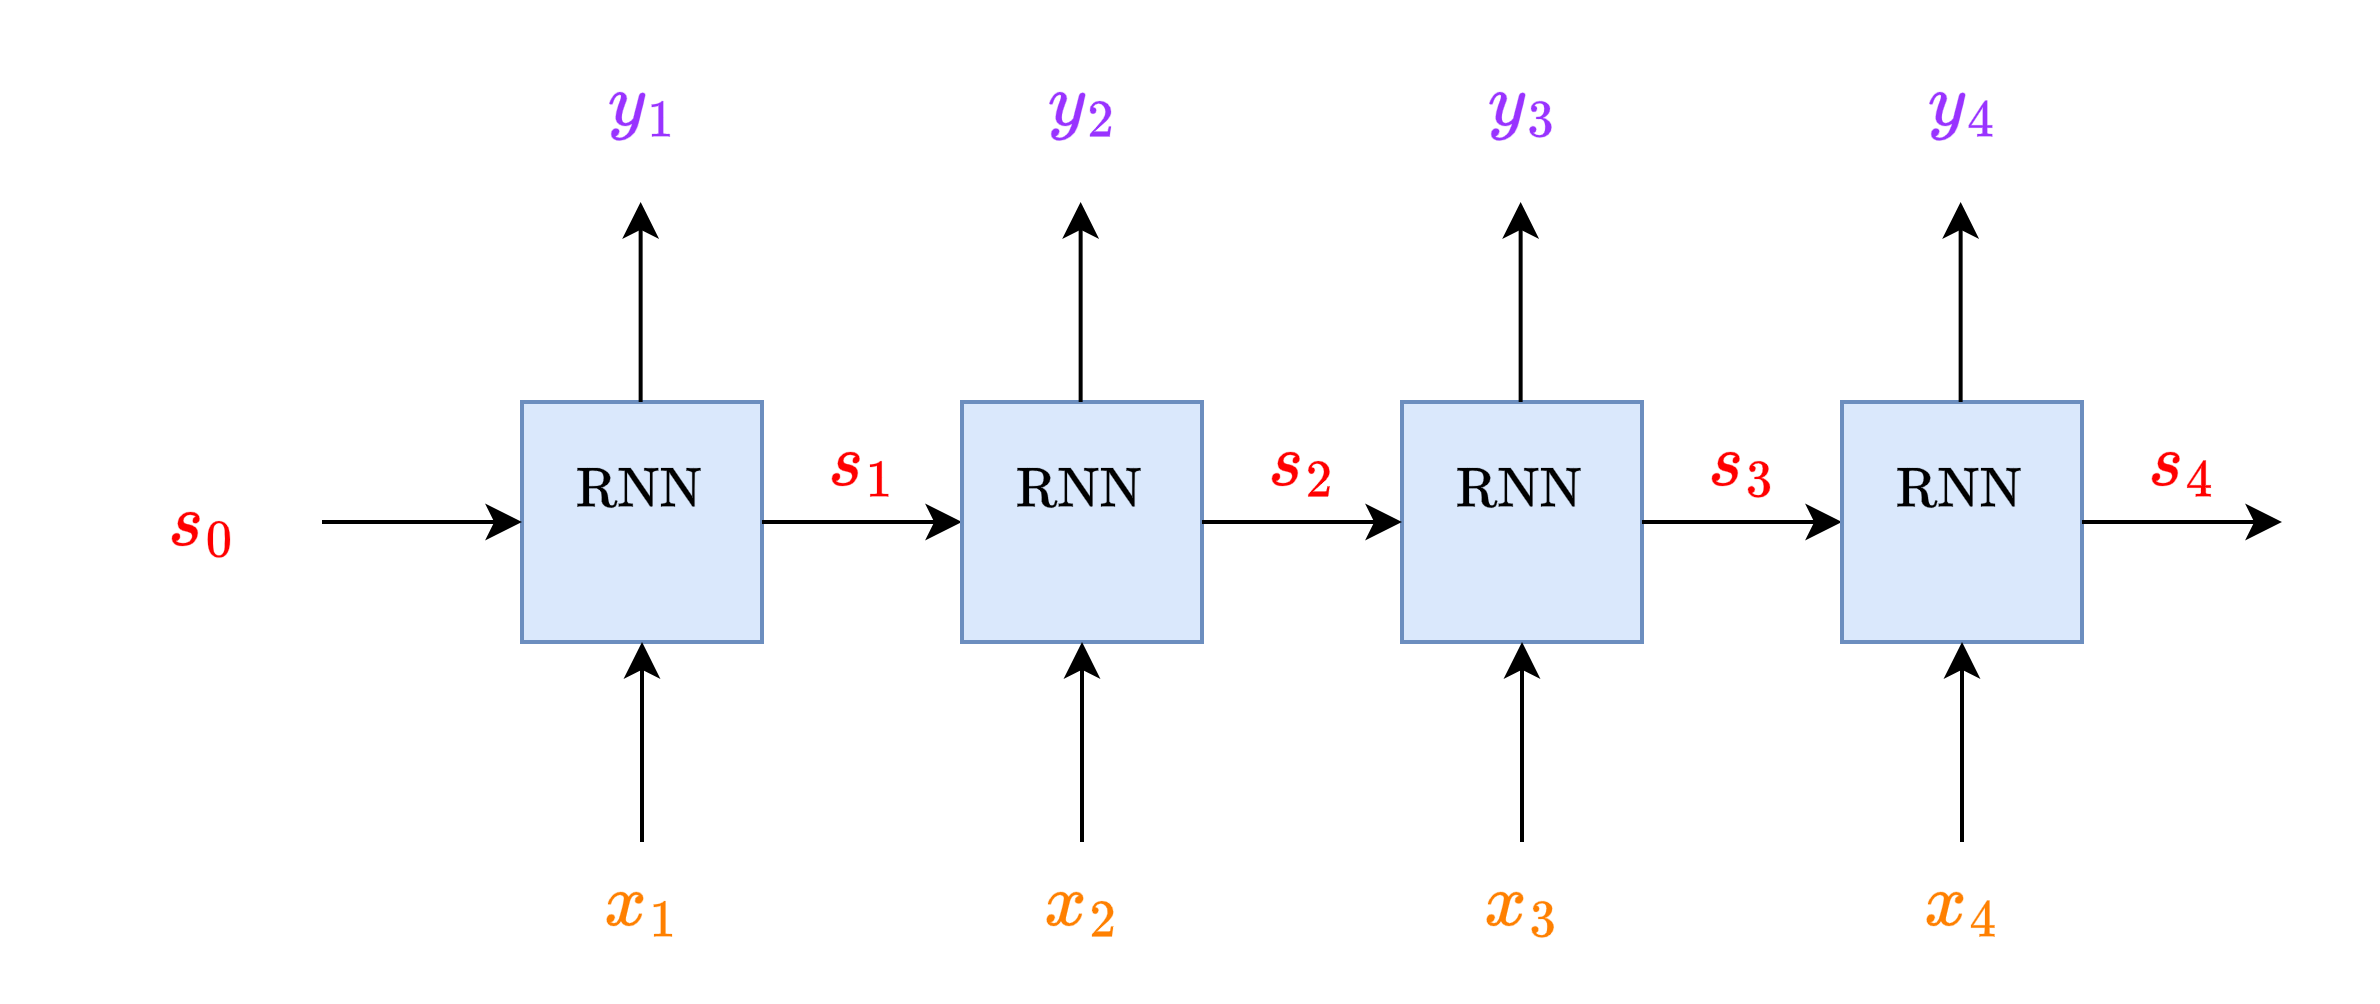
\includegraphics[width=100mm]{images/rnn_images/rnn_simple_layers.png}
            \caption*{In this view, we see a "sequence" of inputs $x_t$, and a "sequence" of outputs $y_t$.}
        \end{figure}
    
        This is why we might call the RNN problem a \vocab{sequence-to-sequence} problem.\\
    
        \begin{concept}
            Rather than seeing each $x_t$ term as an isolated input, we could consider our input the full \purp{sequence}
    
            \begin{equation*}
                x = 
                \begin{bmatrix}
                    x_1 & x_2 & x_3 & \cdots & x_n
                \end{bmatrix}
            \end{equation*}
    
            Our RNN takes the sequence $x$ and returns a paired, output sequence $y$:
    
            \begin{equation*}
                y = 
                \begin{bmatrix}
                    y_1 & y_2 & y_3 & \cdots & y_n
                \end{bmatrix}
            \end{equation*}
    
            In this view, we can think of our RNN as a machine that takes in one sequence, and outputs a second, \gren{equal-length} sequence.

            \subsecdiv

            \begin{itemize}
                \item Notice that $x_t$ and $y_t$ can be \gren{vectors}: $x$ and $y$ may need to be complete \purp{matrices}, to store all these vectors.
            \end{itemize}
        \end{concept}
    
        In this view, we "lump together" all of our inputs and outputs as a single object:
    
        \begin{figure}[H]
            \centering
            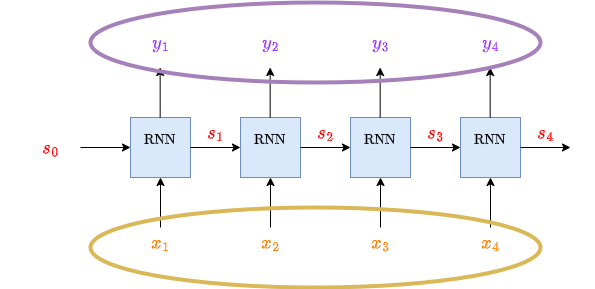
\includegraphics[width=65mm]{images/rnn_images/gathered_sequence.png}
            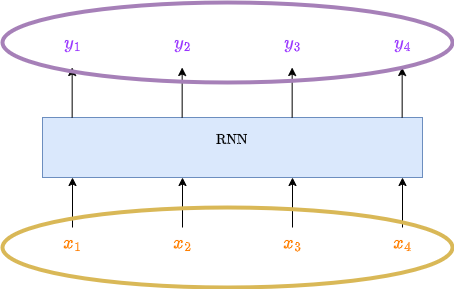
\includegraphics[width=50mm]{images/rnn_images/rnn_seq2seq.png}
    
            \caption*{If we ignore the internal states, our RNN just turns one sequence into another.}
        \end{figure}

        We sometimes call this process \vocab{transduction}.\\

        \begin{definition}
            We say can that our RNN \vocab{transduces} our \brow{input} sequence into our \purp{output} sequence.
        \end{definition}

        Now, we can have \purp{multiple sequences}: for example, we could have our input be, $x=[1,2,3,4]$, or $x=[2,4,6,7]$. Both are valid inputs.
        
        \begin{itemize}
            \item And in each of those sequences, you have \gren{multiple timesteps}.
                \note{And each vector $x_t$ can have multiple elements! We'll ignore this last bit, for our sanity.}
        \end{itemize} 
            

        We'll need to distinguish between these two: difference sequences, versus different timesteps, within a sequence.

        \begin{itemize}
            \item For this purpose, we re-use data point notation $\ex{x}{i}$ that we developed in earlier chapters, Regression and Classification.\\
        \end{itemize}

            
            

        \begin{notation}
            We use $x_t$ to distinguish between inputs in the \gren{same sequence}.

            \begin{itemize}
                \item We'll represent a whole sequence with $x$.
            \end{itemize}

            We'll use $\ex{x}{i}$ to distinguish between \purp{different sequences}.
        \end{notation}

        \begin{itemize}
            \item \miniex $x_3^{(2)}$ is the 3rd timestep, of the 2nd sequence ("data point").
        \end{itemize}

    \phantom{}

    \subsection{Sequence length}
    
        One important observation: we \textbf{need} an input $x_t$ in order to proceed to the next output.

        \begin{itemize}
            \item So, we only have as many outputs as we have inputs.\\
        \end{itemize}

        \begin{concept}
            The \brow{input} and \purp{output} sequences to an RNN will be the \gren{same length}.
        \end{concept}

        What about two different input sequences? 

        \begin{itemize}
            \item Our RNN is capable of taking in sequences of \purp{any length}: if a sequence is longer, we just run our RNN for more timesteps.
        \end{itemize}

        So, each sequence our RNN receives can whatever length it wants to be: they don't have to match length.\\

        \begin{concept}
            An RNN can receive input sequences of \vocab{any length}.

            In fact, the length can be different between \purp{different input sequences}.

            \begin{itemize}
                \item So, sequence $\ex{x}{1}$ and sequence $\ex{x}{2}$ can be used by the \gren{same RNN}, even if they have different lengths.
            \end{itemize}

            \subsecdiv

            This means that each data point needs a separate variable for length: the length of $\ex{x}{i}$ is $\ex{n}{i}$
            
        \end{concept}

        However, we need to be careful of the difference between these two ideas:\\

        \begin{clarification}
            The output sequence $\ex{y}{i}$ \textbf{must} have the \gren{same length} as its input $\ex{x}{i}$: they're \orgg{paired} together.

            However, different inputs ($\ex{x}{i}$ and $\ex{x}{j}$) can have \purp{different lengths}.

            \subsecdiv
            
            This also means that inputs and outputs which are \orgg{not from the same pair} ($\ex{x}{i}$ and $\ex{y}{j}$) can have different lengths.
        \end{clarification}

            \note{Note that this also means that different outputs can have different lengths, as well.}

    \pagebreak
    \subsection{Training data}

        Just like any other NN, we usually are training our RNN for a \textbf{task}. What kind of task?

        \begin{itemize}
            \item The output of our RNN is a \textbf{sequence}: so, our goal will be to take the input sequence $\ex{x}{i}$, and give the \textit{desired} sequence $\ex{y}{i}$.\\
        \end{itemize}

        \begin{concept}
            Training our RNN is similar to our previous model training problems, like \textbf{regression}:

            \begin{itemize}
                \item Given a particular input sequence $\ex{x}{i}$, we want to teach our model to produce the output sequence $\ex{y}{i}$.
            \end{itemize}

            This is similar to regression, where we want to take an input vector, and get a real number as an output.

        \end{concept}

        We want to use this model for \purp{supervised} learning: we know the sequence we want to get as an output.\\

        \begin{definition}
            Our RNN is trained with a \vocab{training set} with $q$ data points:

            \begin{equation*}
                \begin{bmatrix}
                    \quad (\ex{x}{1}, \ex{y}{1}) && (\ex{x}{2}, \ex{y}{2}) && \cdots && (\ex{x}{q}, \ex{y}{q}) \quad \quad
                \end{bmatrix}
            \end{equation*}

            Where, due to the behavior of RNNs (described above), we require:

            \begin{itemize}
                \item Each element $\ex{x}{i}$ or $\ex{y}{j}$ is a \orgg{sequence}.
                
                \item Elements $(\ex{x}{i}, \ex{y}{i})$ from the \gren{same pair} must have the \purp{same length} $\ex{n}{i}$.

                \item \gren{Different pairs} may have \purp{different lengths}. 
                    \begin{itemize}
                        \item Meaning, $\ex{n}{i}$ and $\ex{n}{j}$ are allowed to be different.
                    \end{itemize}
            \end{itemize}
        \end{definition}


        One important note: Now, we're using $y$ to represent the \purp{desired} output, which is not necessarily the same as what our RNN actually gives us.

        \begin{itemize}
            \item We'll need separate notation for this.\\
        \end{itemize}

        \begin{notation}
            From this point on, we'll use \purp{$y$} to indicate the \purp{desired, correct} output, and \gren{$g$} to represent the \gren{current RNN} output.

            \begin{itemize}
                \item So, our goal is to make $g$ and $y$ as \orgg{similar} as possible.
            \end{itemize}
        \end{notation}

        \begin{figure}[H]
            \centering
            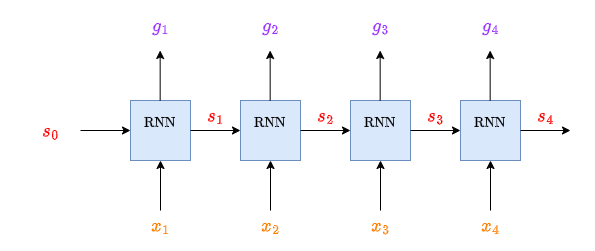
\includegraphics[width=100mm]{images/rnn_images/rnn_simple_g_notation.png}
            \caption*{Very little changes: we just replace $y$ with $g$.}
        \end{figure}




    \phantom{}

    \subsection{Training and Evaluation}

        The desired training output is $\ex{y}{i}$: we will \gren{predict} it using the RNN output, $\ex{g}{i}$.

        \begin{itemize}
            \item For training and evaluation, we'll need a \purp{loss function} to indicate how wrong our guess $\ex{g}{i}$ is.
        \end{itemize}

        This loss will be indicated by $\loss_{seq} \Big(\ex{g}{i}, \ex{y}{i} \Big)$: typically, it will tell us how \gren{different} our sequences are.

        \begin{itemize}
            \item The easiest way to compare two sequences is to compare them \orgg{element-wise}: compare the $\nth{t}$ element of $\ex{y}{i}$ to the $\nth{t}$ element of  $\ex{g}{i}$.\\
        \end{itemize}

        \begin{definition}
            We compute the \vocab{loss} $\loss_{seq}$ of our sequence by adding up the loss $\loss_{elt}$ for each \purp{element} in our sequence.

            \begin{equation*}
                \loss_{seq} \Big(
                    \ex{g}{i}, \ex{y}{i} 
                \Big) = 
                \sum_{ \red{t=1} }^{\red{\ex{n}{i}}} 
                \loss_{elt} \Big( 
                    \ex{g_{\red{t}} }{i}, \ex{y_{\red{t}} }{i} 
                \Big)
            \end{equation*}

            The choice of loss function $\loss_{elt}$ depends on the data type of $\ex{y}{t}$.
        \end{definition}

        \begin{itemize}
            \item Note that for sequence $\ex{g}{i}$, we have $\ex{n}{i}$ timesteps.
        \end{itemize}

        \miniex If our sequence is a series of numbers, we could take the \vocab{squared error} between the elements:

        \begin{equation}
            \ex{g}{i} = 
            \red{
            \begin{bmatrix}
                1 & 4 & 5 
            \end{bmatrix}
            }
            \qquad
            \ex{y}{i} =
            \blu{
            \begin{bmatrix}
                1 & 2 & 3 
            \end{bmatrix}
            }
            \qquad 
            \loss_{elt}(a,b) = (a-b)^2
        \end{equation}

        If compute the total loss, we get

        \begin{equation*}
            \loss_{seq} \Big(
                \ex{g}{i}, \ex{y}{i} 
            \Big) 
            = 
            \sum_{ t=1 }^{3} \Big( 
                \ex{g_{t} }{i}- \ex{y_{t} }{i} 
            \Big)^2 
            =  
            (\red{1}-\blu{1})^2 + (\red{4}-\blu{2})^2 +
            (\red{5}-\blu{3})^2 
        \end{equation*}

        \begin{equation}
            \loss_{seq} \Big(
                \ex{g}{i}, \ex{y}{i} 
            \Big) 
            =
            8
        \end{equation}

        Next, we'll compute the overall performance of our RNN. First, some notation:\\

        \begin{notation}
            We'll collectively represent all of our weights with a $W$:

            \begin{equation*}
                W =\Big( W^{sx}, W^{ss}, W^o, W^{ss}_0, W_0^o \Big)
            \end{equation*}

            These are the \gren{parameters} of our RNN -- they're used for computing $\ex{g}{i}$. Meanwhile, $\ex{x}{i}$ is the \brow{input}, so we find:

            \begin{equation*}
                \ex{g}{i} = RNN \Big( \bro{\ex{x}{i}}; \grn{W}  \Big)
            \end{equation*}
        \end{notation}

        Just like in other problems, we evaluate our model by taking the \vocab{average} of all of our losses:\\

        \begin{definition}
            The \vocab{objective function} $J(W)$ of our RNN is given by \purp{averaging} the loss for each of our $q$ data points:

            \begin{equation*}
                J(W) 
                \quad=\quad 
                \frac{1}{q} \sum_{i=1}^q \loss_{seq} \Big(
                    \ex{g}{i}, \ex{y}{i} 
                \Big) 
                \quad = \quad
                \frac{1}{q} \sum_{i=1}^q \loss_{seq} \Big(\;
                    \overbrace{RNN \Big( \bro{\ex{x}{i}}, \grn{W}  \Big)
                    }^{\ex{g}{i}}
                    \;, \ex{y}{i} 
                \;\Big) 
            \end{equation*}
        \end{definition}



    \phantom{}

    \subsection{Activation Functions}

        Lastly, we want to address our activation functions, $f_s$ and $f_o$.

        $f_s$ is used for our \redd{state}: because our state doesn't directly compute our output, we tend to use the same $f_s$ for different problems:\\

        \begin{concept}
            Our most typical choice for $f_s$ is the \vocab{hyperbolic tangent} function $\tanh$:

            \begin{equation*}
                f_s(z) = \tanh(z) = \frac{e^z-e^{-z}}{e^z+e^{-z}}
            \end{equation*}

            A function whose output ranges over $(-1,+1)$.
        \end{concept}

        \begin{figure}[H]
            \centering
            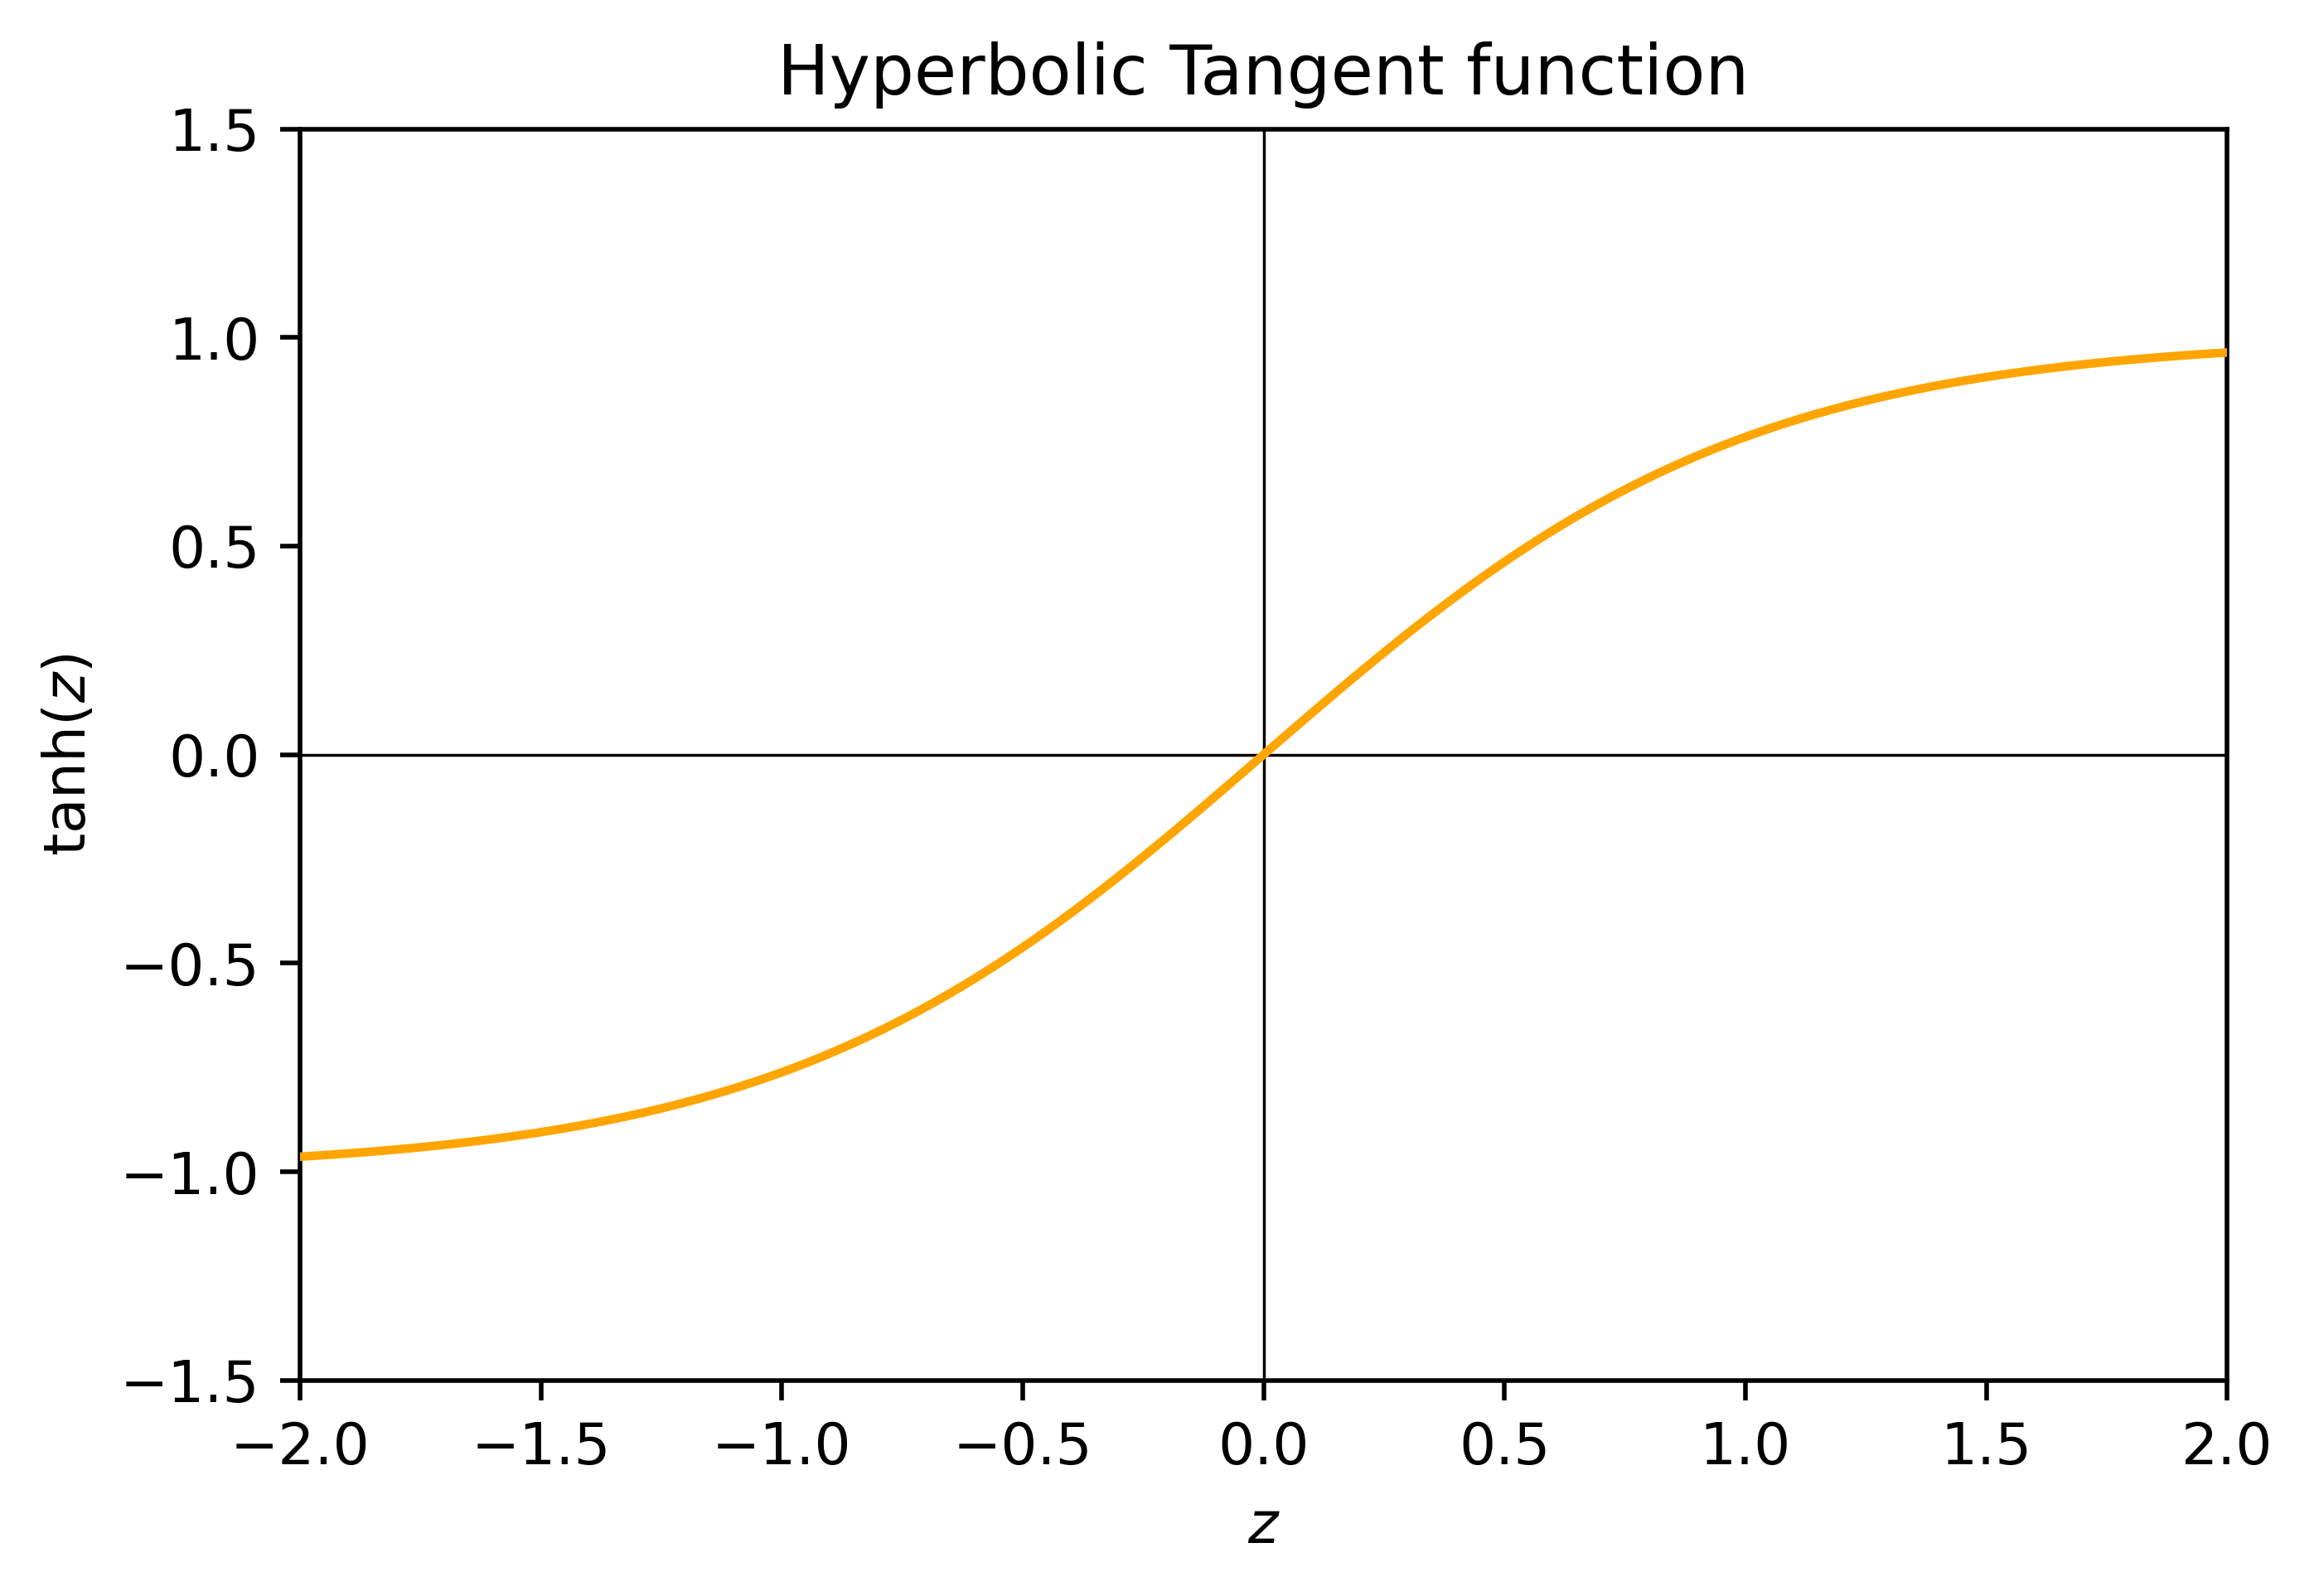
\includegraphics[width=65mm]{images/nn_images/tanh_fn.png}
    
            \caption*{A reminder of how tanh appears: it looks relatively similar to sigmoid, with a different output range.}
        \end{figure}

        Meanwhile, $f_o$ directly allows us to compute the output, so our choice of $f_o$ depends on our problem and data type.\\

        \begin{concept}
            Just like in regular supervised learning, $f_o$ is chosen based on the problem at hand, considering:

            \begin{itemize}
                \item Data type
                \item Range
                \item Sensitivity
            \end{itemize}

            And other properties.
        \end{concept}




\pagebreak

\section{RNN as a language model}

    Human language is written/spoken \gren{sequentially}, with each character/word/syllable coming in a particular \purp{order}.

    Thus, we might expect RNNs, a "sequential" model, to be suited for this task.
        \note{Not nearly as well as transformers, but we'll discuss that in the Transformers chapter.}

    The task in question is \redd{predictive text}:\\

    \begin{definition}
        In the \vocab{predictive text} problem, you're given the "past" sequence of text, and you're supposed to predict "future" text.
    \end{definition}

    \miniex Autocorrect is a common application: based on the words you've typed so far, your phone will predict the most likely next word.

    RNNs can be trained to accomplish this type of task.



    \phantom{}

    \subsection{Tokens}

        Our goal is to \purp{correctly} predict the next word in a sentence, based on the previous words in a sentence.

        First, we'll break up our sentence into a sequence of \textbf{elements}: these elements will be called \vocab{tokens}.\\

        \begin{definition}
            A \vocab{token} is a single \purp{unit} of our text: this might be a single letter/\gren{character}, or a single \gren{word}.
        \end{definition}
        
            \note{Some systems, like chatgpt, will use several characters as a single "token": this set of characters might not line up with each word!}

        \miniex The following sentence contains 3 tokens if a token is a \purp{word}, and 11 tokens if a token is a \gren{character}:

        \begin{equation}
            \begin{matrix}
                1&2&3\\
                \red{I}&\blu{love}&\grn{dogs}
            \end{matrix}
        \end{equation}
        
        \begin{equation}
            \begin{array}{ccccccccccc}
                1 & 2 & 3 & 4 & 5 & 6 & 7 & 8 & 9 & 10 & 11 \\
                \red{I} & \_ & \blu{l} & \blu{o} & \blu{v} & \blu{e} & \_ & \grn{d} & \grn{o} & \grn{g} & \grn{s} \\
            \end{array}
        \end{equation}

        We can represent our sentence $c$ as sequence of tokens $c_i$:

        \begin{equation}
            c = \begin{bmatrix}
                c_1 & c_2 & \cdots & c_k
            \end{bmatrix}
        \end{equation}



    \phantom{}

    \subsection{Predicting tokens}

        We want our RNN to predict \purp{future} tokens in the sentence, based on \gren{past} tokens.  


        \begin{itemize}
            \item Let's start by feeding in our first token:

            \begin{equation}
            RNN\Bigg(\begin{bmatrix}
                \red{c_1}
            \end{bmatrix}\Bigg)
            =
            \begin{bmatrix}
                \blu{G_2}
            \end{bmatrix}
        \end{equation}

        We want our RNN to predict the \gren{next} character, so the \purp{output} will be our prediction for $c_2$: we'll call it $G_2$.\\

        \begin{notation}
            Our \vocab{prediction} for the $\nth{n}$ token, $c_n$, is $G_n$.

            \begin{itemize}
                \item Thus, $G_n$ is the token we consider \gren{most likely}for $c_n$.
            \end{itemize}
        \end{notation}

            \note{Alternatively, $G_n$ could be a vector, giving the \purp{probability} for each possible token that $c_n$ could be.
            
            \phantom{}
            
            This would be useful for evaluating our model: how sure was it of the right answer?}

        


        \phantom{}

        \phantom{}

        \item Let's try our second token:

        \begin{equation}
            RNN\Bigg(\begin{bmatrix}
                \red{c_1} & \blu{c_2}
            \end{bmatrix}\Bigg)
            =
            \begin{bmatrix}
                \blu{G_2} & \grn{G_3}
            \end{bmatrix}
        \end{equation}
        \end{itemize}

        

        

        \phantom{}

        Note that our model gets to see the correct $c_2$, \gren{after} making its prediction, $G_2$.

        \begin{itemize}
            \item That means that our RNN has only seen \red{$c_1$} when it predicts \blu{$G_2$}: it doesn't know what the correct character, \blu{$c_2$}, is yet.

            \item Meanwhile, \grn{$G_3$} is generated with knowledge of \red{$c_1$} and \blu{$c_2$}: the RNN knows what the first two characters are.\\
        \end{itemize}

        

        \begin{concept}
            When our RNN \purp{guesses} the $\nth{t}$ token, $G_t$, it can only see the \gren{first $t-1$ inputs}:

            \begin{equation*}
                \begin{bmatrix}
                    \red{c_1} & \blu{c_2} & \cdots & \org{c_{t-1}}
                \end{bmatrix}
                \quad \xRightarrow[]{RNN} \quad
                \grn{G_{t}}
            \end{equation*}

            Information stored in $c_t$ or $c_{t+1}$, for example, has \orgg{no effect} on $G_t$.

            \begin{itemize}
                \item Otherwise, our model could cheat, and predict by looking at the answer!
            \end{itemize}
        \end{concept}

        In this way, we can supply our entire input, and get a full vector of predictions:

        \begin{equation}
            RNN 
            \Bigg(
            \begin{bmatrix}
                \red{c_1} & \blu{c_2} & \cdots & \org{c_{k-1}} & \grn{c_{k}}
            \end{bmatrix}
            \Bigg)
            \quad=\quad 
            \begin{bmatrix}
                \blu{G_2} & \cdots & \org{G_{k-1}} & \grn{G_{k}} & ?
            \end{bmatrix}
        \end{equation}

        Let's show this in our simplified RNN diagram.
            \note{Remember, the arrows left-to-right are states: they represent all of the previous words in the sentence.}

        \begin{figure}[H]
            \centering
            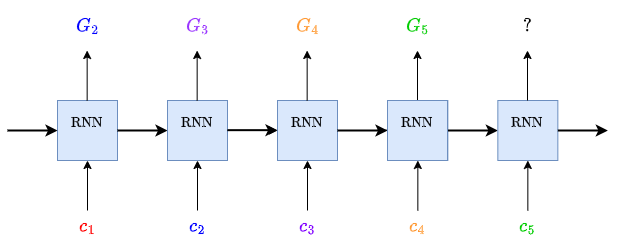
\includegraphics[width=90mm]{images/rnn_images/rnn_predict_text.png}
        \end{figure}

        Here's an example sentence we could try to predict:

        \begin{figure}[H]
            \centering
            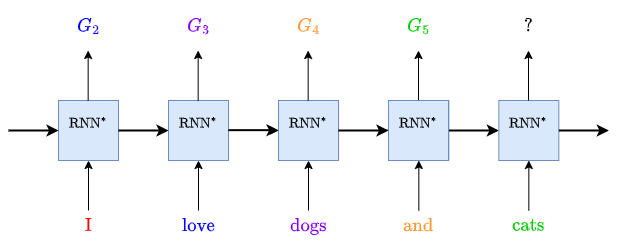
\includegraphics[width=90mm]{images/rnn_images/rnn_predict_example.png}
        \end{figure}

        And now, here's an ideal case, where our RNN performs perfectly (we'll call it RNN$^*$):

        \begin{figure}[H]
            \centering
            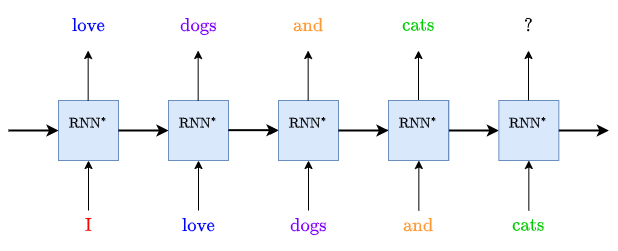
\includegraphics[width=90mm]{images/rnn_images/rnn_predict_soln.png}
            \caption*{Our RNN predicts the right word, right before it appears.}
        \end{figure}

        

    \phantom{}

    \subsection{Start token and end token}

        There are two problems we'd like to fix.

        \begin{itemize}
            \item We'd like to try predicting the first character, $c_1$, rather than \orgg{skipping} it.
            \item If we start with $c_2$, there are only \red{$k-1$} characters we need to predict.
            
                \begin{itemize}
                    \item We have $k$ inputs, and therefore $k$ outputs: we have \gren{one more output} than we need.
                \end{itemize}
        \end{itemize}

        \phantom{}

        Our first solution is to add a special "\purp{START}" token to the beginning of our input:

        \begin{equation}
            x = \begin{bmatrix}
                \purp{START} & c_1 & c_2 & \cdots & c_k
            \end{bmatrix}
        \end{equation}

        What does this do for us?

        \begin{itemize}
            \item During our first timestep, our RNN has nothing other than the \purp{START} token, so it's able to spent that timestep \gren{predicting $c_1$}.
        \end{itemize}

        \begin{equation}
            RNN\Bigg(\begin{bmatrix}
                \purp{START}
            \end{bmatrix}\Bigg)
            =
            \begin{bmatrix}
                g_1
            \end{bmatrix}
        \end{equation}

        Now, our output starts with $G_1$.

        \begin{equation*}
            RNN 
            \Bigg(
            \begin{bmatrix}
                \purp{START} & \red{c_1} & \blu{c_2} & \cdots & \org{c_{k-1}} & \grn{c_{k}}
            \end{bmatrix}
            \Bigg)
            \quad=\quad 
            \begin{bmatrix}
                \red{G_1} & \blu{G_2} & \cdots & \org{G_{k-1}} & \grn{G_{k}} & ?
            \end{bmatrix}
        \end{equation*}

        \begin{definition}
            The \brow{input} to our \vocab{sentence-prediction RNN} starts with the special \purp{START} token, followed by all of the tokens in our sentence $c$.

            \begin{equation*}
                x = \begin{bmatrix}
                    \purp{START} & c_1 & c_2 & \cdots & c_k
                \end{bmatrix}
            \end{equation*}

            \phantom{}

            When our RNN receives this \purp{START} token, it has an opportunity to predict the \orgg{first word} in the sentence, with no context.
        \end{definition}

        \phantom{}

        This hasn't fixed our other problem, though: now we have $k+1$ slots, but only $k$ outputs we need to predict.

        We'll solve that by adding an \redd{END} character at the end of the output.

        \begin{equation}
            y = \begin{bmatrix}
                c_1 & c_2 & \cdots & c_k & \redd{END}
            \end{bmatrix}
        \end{equation}

        \begin{itemize}
            \item Now, we have a desired final output: we want our RNN to predict when the sentence ends, and return \redd{END}.\\
        \end{itemize}

        \begin{definition}
            The \purp{optimal output} of our \vocab{sentence-prediction RNN} starts with all the tokens in our sentence $c$, followed by the special \redd{END} token.
            \begin{equation*}
                y = \begin{bmatrix}
                    c_1 & c_2 & \cdots & c_k & \redd{END}
                \end{bmatrix}
            \end{equation*}
        
        \end{definition}

        Thus, we've fully formed our problem statement:\\

        \begin{concept}
            The goal of our sentence-prediction RNN is to \vocab{replicate the sentence $c$}, token-by-token, with two caveats:

            \begin{itemize}
                \item The input starts with the special \purp{START} token, to give your model one timestep to \gren{predict the first token} $c_1$.
                \item The output should terminate with the special \redd{END} token: your model should \orgg{predict when the sentence ends}.
            \end{itemize}
        \end{concept}


        \begin{figure}[H]
            \centering
            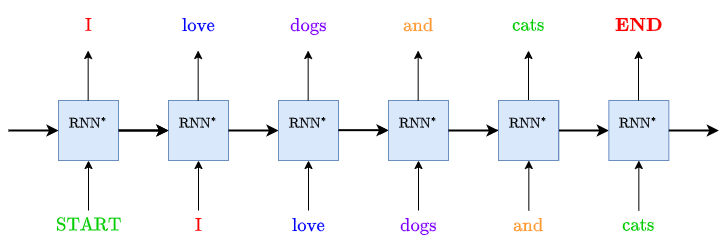
\includegraphics[width=100mm]{images/rnn_images/rnn_predict_startend.png}
            \caption*{Here's what our system looks like, now that we've added the START and END tokens.}
        \end{figure}

        Let's review what happens at each timestep.

        \begin{itemize}
            \item On the bottom, we \gren{input} one word in the sentence.

            \item On the top, we \purp{output} the predicted next word.

            \item After an input, we update our \redd{state}, to include new info. This is \purp{used} by the RNN in the next timestep (left-to-right).
        \end{itemize}









    \pagebreak

    \subsection{Why we might use RNNs for language}

        The general reason we decided to try using RNNs for language is pretty basic:
        
        \begin{itemize}
            \item "RNNs \purp{output sequences}. Text is a \gren{sequence of tokens}".
        \end{itemize}

        \phantom{}

        But there's a bit more to it than that: RNNs allow our model to remember the \orgg{structure} of our sentence, using our \redd{state $s_t$}.

        \begin{itemize}
            \item The newest token $c_t$ might be related to one that we saw \purp{earlier}: for example, 5 tokens ago. 

            \item Our state can treat words that are \gren{closer}, differently from words which are \purp{further away}.
        \end{itemize}

        This way, our \redd{state} allows us to keep track of sentence structure: grammar, the meaning of each word, tone, etc.\\

        \begin{concept}
            When we use an RNN as a \vocab{language model}, we're hoping that it can distinguish between "\gren{nearby}" words, and "\purp{farther away}" words.

            \begin{itemize}
                \item Words which are closer/further can contribute differently to the sentence: this gives us \orgg{context}.
            \end{itemize}
        \end{concept}

        Convolution has a similar effect, but in a more \gren{discrete} way: in convolution, we have a window of a \purp{fixed size}. 
        
        \begin{itemize}
            \item If $n$ is our window size, but two tokens are $n+1$ units apart, then they won't show up together in convolution.
        \end{itemize}

        Meanwhile, RNNs are more flexible:\\

        \begin{concept}
            Depending on how your \redd{RNN state} works, it could preserve/accumulate data over \gren{longer, non-fixed} distances than \purp{convolution}.
        \end{concept}

        \begin{itemize}
            \item \miniex A \gren{running average} could factor in newer information, with older information, without completely "forgetting" that old information.
        \end{itemize}


    \phantom{}

    \subsection{Why RNNs don't work (well) for language}

        Unfortunately, RNNs tend not to work well enough.
        
        \begin{itemize}
            \item Their state $s_t$ can only store a \gren{limited} amount of data.

            \item So, the longer the RNN runs, the more it forgets.\\
        \end{itemize}

        \begin{concept}
            Over time, an RNN will "\purp{forget}" information it learned in \gren{earlier} timesteps.

            \begin{itemize}
                \item It's replaced by \gren{newer} data.
            \end{itemize}
        \end{concept}

        Language requires this sort of longer-term memory.
        
        \begin{itemize}
            \item The longer the text prompt becomes, the worse the RNN performs.
        \end{itemize}

        In the next chapter, we'll design a model to overcome this problem: the \vocab{transformer}.




\pagebreak

\section{Terms}

    \begin{itemize}
        \item Timestep $t$(Review)
        \item State $s_t$
        \item Input $x_t$
        \item Transition function $f_s$
        \item Output $y_t$
        \item Output function $f_o$
        \item State Machine
        \item Finite State Machine
        \item State Transition Diagram
        \item Linearity 
        \item Time-Invariance
        \item Linear Time-Invariant System (LTI)
        \item Recurrent Neural Network (RNN)
        \item Weights $W^{ss}$, $W^{sx}$, $W^{ss}_0$, $W^o$, $W^o_0$
        \item Transduction
        \item $x_t$ notation
        \item $\ex{x}{i}$ notation (Review)
        \item Sequence loss $\loss_{seq}$
        \item Hyperbolic Tangent Function tanh (Review)
        \item Predictive Text
        \item Token
        \item Start Token 
        \item End Token
    \end{itemize}
        

        

        

        

        




        

\iffalse

        
%%%%%%%%%%%%%%%%%%%%%%%%%%%%%%%%%%%%%%%%%%%%%%%%%%%%%%%%%%%%%%%%%%%%%%%%%%%%%

\section{OLD MATERIALS}


%%%%%%%%%%%%%%%%%%%%%%%%%%%%%%%%%%%%%%%%%%%%%%%%%%%%%%%%%%%%%%%%%%%%%%%%%%%%%

% \begin{noticebox}
%   The following material on back-propagation through time
%   (Section~\ref{sec:bptt}) and vanishing gradients and gating
%   mechanisms (Section~\ref{sec:rnn_lstm}) is for your own elucidation.
%   It is not being covered in the Fall 2021 semester of 6.036, and will
%   not be included in the final exam.
% \end{noticebox}

\section{Back-propagation through time}
\label{sec:bptt}

Now the fun begins!  We can now try to find a $W$ to minimize $J$
using gradient descent.  We will work through the simplest method,
{\em back-propagation through time}\index{backpropagation through
  time} ({\sc bptt}), in detail.  This is generally not the best
method to use, but it's relatively easy to understand.  In
Section~\ref{lstm} we will sketch alternative methods that are in much
more common use.

\bigskip 
\begin{noticebox}
  What we want you to take away from this section is that, by
  ``unrolling'' a recurrent network out to model a particular
  sequence, we can treat the whole thing as a feed-forward network
  with a lot of parameter sharing.  Thus, we can tune the parameters
  using stochastic gradient descent, and learn to model sequential
  mapgrngs.  The concepts here are very important.  While the details
  are important to get right if you need to implement something, we
  present the mathematical details below primarily to convey or
  explain the larger concepts.
\end{noticebox}


\begin{examplebox} {\bf Calculus reminder: total derivative} Most of
  us are not very careful about the difference between the {\em
    partial derivative} and the {\em total derivative}\index{total derivative}.  We are going
  to use a nice example from the Wikipedia article on partial
  derivatives to illustrate the difference.

The volume of a circular cone depends on its height and radius:
\begin{equation}
V(r, h) = \frac{\pi r^2 h}{3}\;\;.
\end{equation}
The partial derivatives of volume with respect to height and radius
are
\begin{equation}
\frac{\partial V}{\partial r} = \frac{2\pi r
    h}{3}\;\;\;\text{and}\;\;\; 
\frac{\partial V}{\partial h} = \frac{\pi r^2}{3}\;\;.
\end{equation}
They measure the change in $V$ assuming everything is held constant
except the single variable we are changing.
Now assume that we want to preserve the cone's proportions in the sense that the ratio of radius to height stays constant. 
Then we can't really change one without changing the other.  
In this case, we really have to think about the {\em total derivative}. 
If we're interested in the total derivative with respect to $r$, we sum the ``paths'' along which $r$ might influence $V$:
\begin{align}
\frac{dV}{dr} & = \frac{\partial V}{\partial r} + \frac{\partial
  V}{\partial h} \frac{dh}{dr} \\
& = \frac{2 \pi r h}{3} + \frac{\pi r^2}{3} \frac{dh}{dr} 
\end{align}
Or if we're interested in the total derivative with respect to $h$, we consider how $h$ might influence $V$, either directly or via $r$:
\begin{align}
\frac{dV}{dh} & = \frac{\partial V}{\partial h} + \frac{\partial
  V}{\partial r} \frac{dr}{dh} \\
& = \frac{\pi r^2}{3} + \frac{2 \pi r h}{3} \frac{dr}{dh} 
\end{align}

Just to be completely concrete, let's think of a right circular cone
with a fixed angle $\alpha = \tan r / h$, so that if we change $r$ or
$h$ then $\alpha$ remains constant.  So we have $r = h \tan^{-1}
\alpha$;  let constant $c = \tan^{-1} \alpha$, so now $r = c h$.
Thus, we finally have
\begin{align}
\frac{dV}{dr} & = \frac{2 \pi r h}{3} + \frac{\pi r^2}{3} \frac{1}{c} \\
\frac{dV}{dh} & = \frac{\pi r^2}{3} + \frac{2 \pi r h}{3} c \; .
\end{align}

\end{examplebox}

\noindent The {\sc bptt} process goes like this:
\begin{enumerate}[(1)]
\item
Sample a training pair of  sequences $(x, y)$; let their length be $n$.
\item
``Unroll" the RNN to be length $n$ (picture for $n = 3$ below), and
initialize $s_0$:

Now,  we can see our problem as one of performing what is almost an
ordinary back-propagation training procedure in a feed-forward neural
network, but with the difference that the weight matrices are shared
among the layers.  In many ways, this is similar to what ends up
happening in a convolutional network, except in the conv-net, the
weights are re-used spatially, and here, they are re-used temporally.
\item
Do the {\it forward pass}, to compute the predicted output sequence $g$:
\begin{align}
z_t^1 &= W^{sx}x_t + W^{ss}s_{t - 1} + W^{ss}_0\\
s_t &= f_s(z_t^1)\\
z_t^2 &= W^os_t + W_0^o\\
g_t &= f_o(z_t^2)
\end{align}
\item
Do {\em backward pass} to compute the gradients. For both $W^{ss}$ and
$W^{sx}$ we need to find
\begin{align}
\frac{d \mathcal{L}_\text{seq}(g,y)}{d W} &= \sum_{u = 1}^n\frac{d \mathcal{L}_\text{elt}(g_u, y_u)}{d W} ~~~~~~~~~~~~~~~~~~ \nonumber
\end{align}
Letting $\mathcal{L}_u = \mathcal{L}_\text{elt}(g_u, y_u)$ and using the {\em  total derivative}, which is a sum over all
the ways in which $W$ affects $\mathcal{L}_u$, we have
\begin{align}
~~~~ &= \sum_{u = 1}^n\sum_{t = 1}^n  \frac{\partial s_t}{\partial W} \frac{\partial \mathcal{L}_u}{\partial s_t}  \nonumber
\end{align}
Re-organizing, we have
\begin{align}
~~~~ &= \sum_{t = 1}^n\frac{\partial s_t}{\partial W} \sum_{u =
  1}^n\frac{\partial \mathcal{L}_u}{\partial s_t} \nonumber
\end{align}
Because $s_t\ \text{only affects}\ \mathcal{L}_t, \mathcal{L}_{t + 1}, \dots, \mathcal{L}_n$, 
\begin{align}
~~~~~~~~~~~~~~~~~~~~ &= \sum_{t = 1}^n\frac{\partial s_t}{\partial W} \sum_{u = t}^n\frac{\partial \mathcal{L}_u}{\partial s_t} \nonumber\\
&= \sum_{t = 1}^n\frac{\partial s_t}{\partial W} 
  \left(\frac{\partial \mathcal{L}_t}{\partial s_t} + \underbrace{\sum_{u = t +
  1}^n\frac{\partial \mathcal{L}_u}{\partial s_t}}_{\delta^{s_t}}\right) \; .\label{sumeq}
\end{align}
where $\delta^{s_t}$ is the dependence of the future loss (incurred after step $t$) on the
state $S_t$.\note{That is, $\delta^{s_t}$ is how much we can
  blame state $s_t$ for all the future element losses.}

We can compute this backwards, with $t$ going from $n$ down to $1$. 
The trickiest part is figuring out how early states contribute to later
losses. We define the {\it{future loss}} after step $t$ to be
\begin{equation}
F_t = \sum_{u = t + 1}^{n}\mathcal{L}_\text{elt}(g_u, y_u) \;\;,
\end{equation}
so 
\begin{equation}
\delta^{s_t} = \frac{\partial F_t}{\partial s_t}\;\;.
\end{equation}
At the last stage, $F_n = 0$ so $\delta^{s_n} = 0$.

Now, working backwards, 
\begin{align}
\delta^{s_{t -1}} &= \frac{\partial}{\partial s_{t - 1}}\sum_{u = t}^n\mathcal{L}_\text{elt}(g_u, y_u)\\
&= \frac{\partial s_t}{\partial s_{t - 1}} \frac{\partial}{\partial s_t}\sum_{u = t}^n\mathcal{L}_\text{elt}(g_u, y_u)\\
&= \frac{\partial s_t}{\partial s_{t - 1}} \frac{\partial}{\partial s_t}\left[\mathcal{L}_\text{elt}(g_t, y_t) + \sum_{u = t + 1}^n\mathcal{L}_\text{elt}(g_u, y_u)\right]\\
&= \frac{\partial s_t}{\partial s_{t - 1}} \left[\frac{\partial \mathcal{L}_\text{elt}(g_t, y_t)}{\partial s_t} + \delta^{s_t}\right]
\end{align}
Now, we can use the chain rule again to find the dependence of the
element loss at time $t$ on the state  at that same time,
\begin{equation}
  \underbrace{\frac{\partial \mathcal{L}_\text{elt}(g_t,
    y_t)}{\partial s_t}}_{(m \times 1)} = \underbrace{\frac{\partial
    z_t^2}{\partial s_t}}_{(m \times v)} ~
\underbrace{\frac{\partial \mathcal{L}_\text{elt}(g_t, y_t)}{\partial
    z_t^2}}_{(v \times 1)}\;\;, 
\end{equation}
and the dependence of the state at time $t$ on the state at the
previous  time, 
%noting that we are performing an {\em elementwise}
%multiplication between $W^T_{ss}$ and the vector of ${f^1}'$ values, $\partial
%s_t /\partial z^1_t$:
\iffalse
\note{There  are two ways  to think about $\partial s_t  / \partial
  z_t$:  here, we take the view  that it is an $m \times 1$ vector and
  we multiply each column of $W^T$ by it.  Another, equally good,
  view, is that it is an $m \times m$ diagonal matrix, with the values
  along the diagonal, and then  this operation is a matrix multiply.
  Our software implementation will take the first view.
}
\fi
\begin{equation}
  \underbrace{\frac{\partial s_t}{\partial s_{t - 1}}}_{(m \times m)}
= \underbrace{\frac{\partial z_t^1}{\partial s_{t - 1}}}_{(m \times
  m)} \underbrace{\frac{\partial s_t}{\partial z_t^1}}_{(m
  \times m)} = {W^{ss}}^T \frac{\partial s_t}{\partial z_t^1}
\end{equation} \\
\begin{examplebox} Note that $\partial s_t /\partial z^1_t$
is formally an $m \times m$ diagonal matrix, with the values
  along the diagonal being $f_{s}'(z_{t,i}^1)$, $1 \leq i \leq m$. But since this is a diagonal matrix, one could represent it as an $m \times 1$ vector $f_{s}'(z_t^1)$. In that case the product of the matrix ${W^{ss}}^T$ by the vector $f_{s}'(z_t^1)$, denoted ${W^{ss}}^T * f_{s}'(z_t^1)$, should be interpreted as follows: take the first column of the matrix ${W^{ss}}^T$ and multiply each of its elements by the first element of the vector $\partial s_t /\partial z^1_t$, then take the second column of the matrix ${W^{ss}}^T$ and multiply each of its elements by the second element of the vector $\partial s_t /\partial z^1_t$, and so on and so forth ...
\end{examplebox}
  
Putting this all together, we end up with
\begin{equation}
  \delta^{s_{t - 1}} = \underbrace{{W^{ss}}^T \frac{\partial s_t}{\partial z_t^1}}_{\frac{\partial s_t}{\partial s_{t - 1}}} ~ \underbrace{\left({W^o}^T\frac{\partial{\mathcal{L}_t}}{\partial z_t^2} + \delta^{s_t}\right)}_{\frac{\partial F_{t - 1}}{\partial s_t}} 
\end{equation}

We're almost there!  Now, we can describe the actual weight updates.
Using Eq.~\ref{sumeq} and recalling the definition of
$\delta^{s_t} = \partial F_t / \partial s_t$, 
as we iterate backwards, we can accumulate the terms in Eq.~\ref{sumeq}
to get the gradient for the whole  loss.
\iffalse
\begin{align}
\frac{ d \mathcal{L}_\text{seq}}{d W^{ss}} &+= 
\frac{\partial F_{t-1}}{\partial W^{ss}} = 
\frac{\partial z^1_t}{\partial W^{ss}} \frac{\partial s_t}{\partial z^1_t}
\frac{\partial F_{t-1}}{\partial s_t} \\
\frac{ d \mathcal{L}_\text{seq}}{d W^{sx}} &+= 
\frac{\partial F_{t-1}}{\partial W^{sx}} = 
\frac{\partial z^1_t}{\partial W^{sx}} \frac{\partial s_t}{\partial z^1_t}
\frac{\partial F_{t-1}}{\partial s_t} 
\end{align}
\fi



\begin{align}
  \frac{d \mathcal{L}_\text{seq}}{d W^{ss}} & = \sum_{t=1}^n
  \frac{d \mathcal{L}_\text{elt}(g_t, y_t)}{d W^{ss}} = \sum_{t=1}^n \frac{\partial z_t^1}{\partial W^{ss}} \frac{\partial s_t}{\partial z_t^1} \frac{\partial F_{t - 1}}{\partial s_t} \\
  \frac{d \mathcal{L}_\text{seq}}{d W^{sx}} & =  \sum_{t=1}^n                                                          
 \frac{d \mathcal{L}_\text{elt}(g_t, y_t)}{d W^{sx}} = \sum_{t=1}^n
 \frac{\partial z_t^1}{\partial W^{sx}} \frac{\partial s_t}{\partial z_t^1} \frac{\partial F_{t-1}}{\partial s_t} 
 \end{align}
 We can handle $W^o$ separately;   it's easier because it does not
affect future  losses  in the way that the other weight matrices do:
\begin{equation}
  \frac{d\mathcal{L}_\text{seq}}{d W^o} = \sum_{t = 1}^n\frac{d \mathcal{L}_t}{d W^o} = \sum_{t = 1}^n\frac{\partial \mathcal{L}_t}{\partial
  z_t^2} \frac{\partial z_t^2}{\partial W^o} 
\end{equation} 
Assuming we have $\frac{\partial \mathcal{L}_t}{\partial z_t^2} = (g_t - y_t)$,
(which ends up being true for squared loss, softmax-NLL, etc.), then 
\begin{equation}
  \underbrace{\frac{d \mathcal{L}_\text{seq}}{d W^o}}_{v \times m} = \sum_{t=1}^n \underbrace{(g_t - y_t)}_{v \times 1} ~ \underbrace{s_t^T}_{1 \times m} \; .
\end{equation}

Whew!
\end{enumerate}
\question{Derive the updates for the offsets $W^{ss}_0$ and $W^o_0$.}

%%%%%%%%%%%%%%%%%%%%%%%%%%%%%%%%%%%%%%%%%%%%%%%%%%%%%%%%%%%%%%%%%%%%%%%%%%%%%
\section{Vanishing gradients and gating mechanisms}
\label{lstm}
\label{sec:rnn_lstm}

Let's take a careful look at the backward propagation of the gradient
along the sequence:
\begin{equation}
\delta^{s_{t -1}} = \frac{\partial s_t}{\partial s_{t - 1}} ~
  \left[\frac{\partial \mathcal{L}_\text{elt}(g_t, y_t)}{\partial s_t}
    + \delta^{s_t}\right]\;\;.
\end{equation}
Consider a case where only the output at the end of the sequence is
incorrect, but it depends critically, via the weights,  on the input
at time 1.   In this case, we will multiply the loss at step $n$ by 
\begin{equation}
\frac{\partial s_2}{\partial s_1} \frac{\partial s_3}{\partial
    s_2} \cdots \frac{\partial s_n}{\partial s_{n-1}}\;\;.
\end{equation}
In general, this quantity will either grow or shrink exponentially
with the length of the sequence, and make it very difficult to train.
\question{The last time we talked about exploding and vanishing
  gradients, it was to justify per-weight adaptive step sizes.  Why is
  that not a solution to the problem this time?}

An important insight that really made recurrent networks work well on
long sequences is the idea of {\em gating}\index{recurrent neural network!gating}.

\subsection{Simple gated recurrent networks}

A computer only ever updates some parts of its memory on each
computation cycle.  We can take this idea and use it to make our
networks more able to retain state values over time and to make the
gradients better-behaved.  We will add a new component to our network,
called a {\em gating network}\index{gating network}.  Let $g_t$ be a $m \times 1$ vector of
values and let $W^{gx}$ and $W^{gs}$ be $m \times l$ and $m \times m$
weight matrices, respectively.  We will compute $g_t$ as
\note{It can have an offset, too, but we are omitting it for simplicity.}
\begin{equation}
g_t = \text{sigmoid}(W^{gx} x_t + W^{gs} s_{t-1})
\end{equation}
and then change the computation of $s_t$ to be
\begin{equation}
s_t = (1 - g_t) *  s_{t-1} + g_t * s(W^{sx}x_t + W^{ss}
  s_{t-1} + W^{ss}_0)\;\;,
\end{equation}
where $*$ is component-wise multiplication.  We can see, here, that
the output of the gating network is deciding, for each dimension of
the state, how much it should be updated now.  This mechanism makes it
much easier for the network to learn to,  for example, ``store'' some
information in some dimension of the state, and then not change it
during future state updates, or change it only under certain
conditions on the input or other aspects of the state.
\question{Why is it important that the activation function for $g$ be
  a sigmoid?}

\subsection{Long short-term memory}

The idea of gating networks can be applied to make a state machine
that is even more like a computer memory, resulting in a type of
network called an {\sc  lstm}\index{long short-term memory} for ``long short-term memory.''
\note{Yet another awesome name for a neural network!}  We won't go
into the details here,  but the basic idea is that there is a memory
cell (really, our state vector) and three (!) gating networks.  The
{\em input} gate selects (using a ``soft''  selection as in the gated
network above) which dimensions of the state will be updated  with new
values;  the {\em forget} gate decides which dimensions of the state
will have its old values  moved toward 0, and the {\em  output} gate
decides which dimensions of the state will be used to compute the
output value.  These networks have been used in applications like
language translation with really amazing results.  A diagram of the 
architecture is shown below:
\begin{center}
\includegraphics[scale = 0.7]{figures/lstm.png}
\end{center}

\fi


%%% Local Variables:
%%% mode: latex
%%% TeX-master: "top"
%%% End:
